 \documentclass[

12pt, % tamanho da fonte

openright, % capítulos começam sempre em página ímpar

oneside, % impressão só frente (use "twoside" se frente e verso)

a4paper, % papel A4

brazil % idioma principal

]{abntex2}

% Pacotes básicos

\usepackage[utf8]{inputenc} % acentuação

\usepackage[T1]{fontenc} % codificação da fonte

\usepackage{lmodern} % usa fonte Latin Modern

\usepackage{microtype} % melhora a justificação

\usepackage{graphicx} % inserir figuras

\usepackage[alf]{abntex2cite} % citações padrão ABNT

\usepackage{url}

\usepackage{indentfirst} % recuo no primeiro parágrafo

\usepackage{ragged2e} % para justificação

\usepackage{amsmath} % para \text{} e outras paradas de equação

\usepackage{multirow} %para o multirow

\usepackage{float} % necessário para [H]

\usepackage{tikz} %desenho de diagramas

\usepackage{pgfplots}

\usepackage{tikz}

\usetikzlibrary{positioning, shapes.geometric, arrows.meta, arrows}


\pgfplotsset{compat=1.18}


%regras da UESC :X

\usepackage[

letterpaper, % Usa o tamanho de papel padrão (A4 é o padrão na maioria das distribuições modernas, mas 'a4paper' pode ser usado para forçar)

top=3cm, % Margem superior padrão [cite: 2472]

bottom=2cm, % Margem inferior [cite: 2475]

left=3cm, % Margem esquerda [cite: 2473]

right=2cm, % Margem direita [cite: 2474]

headsep=0.5cm % Espaço entre o cabeçalho e o texto (ajuste fino opcional)

]{geometry}


\usepackage{titlesec}

\usepackage{calc}


% Define a formatação das Seções Primárias (1 INTRODUÇÃO, 2 FUNDAMENTAÇÃO TEÓRICA, etc.)

% A UESC exige: 7cm no topo. Títulos em CAIXA ALTA e Negrito.


\titleformat{\section}[block] % block é um estilo adequado para seções numeradas

{

\normalfont\Large\bfseries\MakeUppercase % Estilo: CAIXA ALTA, Negrito, Grande

}

{

\thesection % Número da seção (Ex: 1)

}

{

1em % Espaço entre o número e o título (mantemos 1em, que é o padrão)

}

{

% Comando que insere espaço vertical antes do título (o 7cm é a margem + o que vem antes do título)

\vspace*{\dimexpr 7cm-\topskip-\baselineskip} % Subtrai valores internos do LaTeX

}


% Recuo e espaçamento entre parágrafos (ABNT)

\setlength{\parindent}{1.25cm} % recuo de 1,25 cm

%\setlength{\parskip}{0.2cm} % espaço entre parágrafos -- PACOTES DE CONTEÚDO E RECURSOS ---
\usepackage{graphicx}         % inserir figuras
\usepackage[alf]{abntex2cite}      % citações padrão ABNT
\usepackage{url}  
\usepackage{amsmath} % para \text{} e outras paradas de equação
\usepackage{multirow} % para o multirow
\usepackage{float} % necessário para [H]
\usepackage{pgfplots}
\usepackage{tikz} % desenho de diagramas
\usetikzlibrary{positioning, shapes.geometric, arrows.meta, arrows}

\pgfplotsset{compat=1.18} 

% Recuo e espaçamento entre parágrafos (ABNT)
\setlength{\parindent}{1.25cm} % recuo de 1,25 cm
%\setlength{\parskip}{0.2cm}    % espaço entre parágrafos
% Informações do trabalho

\titulo{Título do seu TCCe}
\autor{João Victor Sousa}
\local{Ilhéus - Bahia}
\data{2025}
\orientador{Otacílio José Pereira}
\instituicao{
  Universidade Estadual de Santa Cruz \par
  Curso de Graduação em Ciênca da Computação}
\tipotrabalho{Trabalho de Conclusão de Curso}
\preambulo{Trabalho apresentado ao Curso de Y da Universidade X como requisito parcial para obtenção do título de Bacharel.}

\begin{document}

% Capa e folha de rosto
\imprimircapa
\imprimirfolhaderosto*

% Resumo
\begin{resumo}
Escreva aqui o resumo do seu trabalho.  
Inclua objetivos, metodologia, resultados e conclusões.

\vspace{\onelineskip}
\noindent
\textbf{Palavras-chave}: palavra1. palavra2. palavra3.
\end{resumo}

% Sumário
\tableofcontents

%lista de tabelas
\newpage
\listoftables

%lista de figuras
\newpage
\listoffigures

\chapter*{Lista de Siglas} 
\begin{tabular}{ll}
AAMI – \textit{Association for the Advancement of Medical Instrumentation}\\
ANN – \textit{Artificial Neural Network}\\
AP – \textit{Average Precision} \\
AUC – \textit{Area Under the Curve}\\
AUPRC – \textit{Area Under the Precision-Recall Curve}\\
BCE – \textit{Binary Cross-Entropy}\\
CNN – \textit{Convolutional Neural Network}\\
ECG – Eletrocardiograma\\
FA – Fibrilação Atrial\\
FC – \textit{Fully Connected}\\
FN – \textit{False Negative}\\
FP – \textit{False Positive}\\
FV – Fibrilação Ventricular \\
GRU – \textit{Gated Recurrent Unit}\\
KNN – \textit{K-Nearest Neighbor}\\
LIME – \textit{Local Interpretable Model-agnostic Explanations} \\
LSTM – \textit{Long Short-Term Memory}\\
MIT-BIH – \textit{Massachusetts Institute of Technology} - \textit{Beth Israel Hospital}\\
OMS – Organização Mundial da Saúde \\
PVC – \textit{Premature Ventricular Contraction} \\
ReLU – \textit{Rectified Linear Unit}\\
RNN – \textit{Recurrent Neural Network}\\
SHAP – \textit{SHapley Additive exPlanations}\\
SMOTE – \textit{Synthetic Minority Over-sampling Technique} \\
SVM – \textit{Support Vector Machine}\\
TN – \textit{True Negative}\\
TP – \textit{True Positive} \\
TSV – Taquicardia Supraventricular\\
TV – Taquicardia Ventricular\\
VEB – \textit{Ventricular Ectopic Beat} \\
\end{tabular}


% Capítulos
\chapter{Introdução}
Texto da introdução.

\chapter{Fundamentação Teórica}
\label{ch:fundamentacao}

Como o trabalho envolve o reconhecimento de arritmias cardíacas, o primeiro ponto é compreender
como o coração funciona, mais especialmente, como o funciona o mecanismo do impulso elétrico responsáveis pela 
contração do mesmo. Em seguida, entender o princípio de funcionamento das redes neurais, que integra a solução 
para o problema. Por fim, será apresentado alguns trabalhos que correlacionaram as duas áreas.

\section{Funcionamento do coração}
\label{sec:funciionamento_coracao}

O coração é um órgão muscular composto por quatro câmaras — átrio direito e esquerdo, e ventrículo direito e esquerdo — que se contraem de forma rítmica, bombeando sangue para o corpo. Essas contrações são controladas por correntes elétricas que percorrem o coração de maneira precisa e em velocidade controlada.

Na Figura~\ref{fig:coracao_esquema_eletrico}, o sistema de condução elétrica do coração é ilustrado.

\begin{figure}[H]
  \centering
  \caption{Sistema de condução do coração}
   \includegraphics[width=0.35\textwidth]{figuras/coracao_sistema_eletrico.png} % insere o tikzpicture puro
  \label{fig:coracao_esquema_eletrico}
    \legend{Fonte: Adaptado de \citeonline{Mitchell_Arritmias_MSD}}
\end{figure}

Segundo \citeonline{Mitchell_Arritmias_MSD}, o batimento cardíaco normal se inicia no nódulo sinusal (1), localizado no átrio direito, que atua como o marcapasso natural do coração. A corrente elétrica propaga-se do átrio direito para o esquerdo (2), promovendo sua contração e o bombeamento do sangue para os ventrículos. Em seguida, o impulso atinge o nódulo atrioventricular (3) — conexão entre os átrios e ventrículos — onde é temporariamente retardado, permitindo que os átrios se contraiam completamente e encham as câmaras inferiores.

Posteriormente, a corrente percorre o feixe de His (4), que se divide e conduz o impulso para ambos os ventrículos (5), promovendo sua contração e o bombeamento do sangue para o restante do corpo.

\section{O eletrocardiograma}
\label{sec:ecg}

O eletrocardiograma, ECG, é um exame não invasivo usado para medir a atividade elétrica do coração. Ele é feito a partir do contato de eletrodos, chamados de derivações ou \textit{leads}, sobre a pele.
A quantidade de eletrodos varia, mas geralmente são 12 \cite{msd_ecg}.

Ao registrar a magnitude e direção da corrente, as derivações geram uma onda que representa a atividade elétrica do coração. O passo a passo descrito em \ref{sec:funciionamento_coracao} é refletido em sua morfologia.

Na Figura~\ref{fig:ecg_exemplo_coracao}, é ilustrado um  ECG de um batimento, observe que ele é subdividido em: onda P, complexo QRS e onda T \cite{msd_ecg}. Note que cada uma dessas partes se refere a um estágio do batimento.

\begin{figure}[H]
  \centering
  \caption{Exemplo de ECG com sua morfologia destacada}
   \includegraphics[width=0.7\textwidth]{figuras/ecg_exemplo_coracao.png} % insere o tikzpicture puro
  \label{fig:ecg_exemplo_coracao}
    \legend{Fonte: Adaptado de  \citeonline{msd_ecg}}
\end{figure}

\section{Arritmias}

As doenças cardíacas podem ser diversas. Dentre elas, as arritmias são um grupo que podem ser diagnósticas via ECG

\subsection{Arritmias clínicas}

As arritmias são alterações no ritmo cardíaco que podem ter diversas causas, incluindo alterações hormonais, uso de medicamentos, toxinas (como álcool ou cafeína), anomalias eletrolíticas ou doenças cardíacas.
Segundo \citeonline{Mitchell_Arritmias_MSD}, em adultos em repouso, a frequência cardíaca normal varia entre 60 e 100 batimentos por minuto (bpm). Frequências mais baixas, conhecidas como bradicardia sinusal, são comuns em atletas, crianças pequenas, adolescentes, jovens adultos e durante o sono. Por outro lado, a taquicardia sinusal ocorre quando a frequência se eleva, podendo ser observada durante o esforço físico, doenças, estimulação neural simpática ou emoção intensa.

Variações no ritmo cardíaco são fenômenos fisiológicos normais. Durante a respiração, por exemplo, é comum que a frequência aumente e diminua levemente, comportamento conhecido como arritmia sinusal respiratória. O autor ainda observa que um ritmo cardíaco perfeitamente regular pode indicar patologias no sistema nervoso autônomo, como ocorre em casos de diabetes avançado. Dessa forma, ainda não existe um indicador global e definitivo do que seria um ritmo sinusal considerado saudável.


As arritmias podem ser classificadas de forma simplificada em três tipos principais:

\begin{enumerate}
    \item \textbf{Taquicardia} — frequência excessivamente rápida;
    \item \textbf{Bradicardia} — frequência excessivamente lenta;
    \item \textbf{Irregular} — quando os impulsos percorrem o coração por vias irregulares.
\end{enumerate}

Observe na Figura~\ref{fig:ecg_exemplo_coracao}, exemplos desses três tipos arrítmicos ilustrados em um ECG.

\subsection{Padrões de classificação para algoritmos (AAMI)}

\label{sub_sec:padroes_arritmias_aami}

A \textit{Association for the Advancement of Medical Instrumentation}, AAMI, define cinco classes de arritmia: normal (N), ventricular (V), supraventricular (S), fusão (F) e não classificado (Q) \cite{silva2025,saadatnejad2020}.

\subsubsection{Arritmias Ventriculares}

As arritmias ventriculares incluem, por exemplo, as contrações prematuras ventriculares (PVCs) e os batimentos de escape. 
O batimento ventricular de escape atua como um mecanismo compensatório, funcionando como um “backup” protetivo do coração quando o marcapasso natural falha temporariamente.
De acordo com \citeonline{Sattar_Premature_2025}, as PVCs são batimentos originários dos ventrículos que podem ocorrer mesmo em indivíduos saudáveis. Sua morfologia é variável, dependendo da origem do impulso, de doenças estruturais ou ainda de uso de medicamentos. Quando frequentes, podem causar fadiga e palpitações, evoluindo para disfunções ventriculares e, em alguns casos, representando a primeira manifestação de cardiopatias estruturais.

\citeonline{msdmanuals_ventricular} cita ainda outras causas potenciais de PVCs, como doenças da artéria coronária (especialmente durante ou após infarto), dilatação ventricular decorrente de insuficiência cardíaca e alterações nas válvulas cardíacas. Em pacientes com doenças estruturais, as PVCs podem progredir para arritmias mais graves, como taquicardia ventricular (VT) e fibrilação ventricular (FV), que representam risco de morte súbita.

\citeonline{mitchell2024afib,mitchell2024vt} descrevem tanto a fibrilação quanto a taquicardia ventricular como arritmias originadas nos ventrículos.

A taquicardia ventricular (TV) produz uma frequência cardíaca de até 120 bpm e é formada por uma sequência de contrações ventriculares prematuras (PVCs). Quando persiste por mais de 30 segundos, recebe a denominação de taquicardia sustentada. Costuma ocorrer em indivíduos com alterações estruturais cardíacas, como infarto do miocárdio, falha cardíaca ou cardiomiopatia. Os sintomas incluem fraqueza, tontura e desconforto torácico. Caso persista por mais de 30 segundos, o tratamento é indicado mesmo na ausência de sintomas, uma vez que pode evoluir para fibrilação ventricular.

Outro tipo de arritmia ventricular é o \textit{flutter} ventricular. Segundo o \citeonline{mesh_ventricular_flutter}, elas são caracterizadas por uma taquicardia extremamente rápida e instável hemodinamicamente (150 a 300 bpm).
São potencialmente fatais e, tipicamente, evoluem para a fibrilação ventricular.

A fibrilação ventricular (FV), por outro lado, é caracterizada por batimentos rápidos e desordenados, resultantes de sinais elétricos caóticos nos ventrículos. Essa condição leva à perda de consciência em poucos segundos e à morte caso não haja intervenção imediata, configurando-se como um tipo de parada cardíaca. Entre suas causas estão afogamentos, choques elétricos e falha cardíaca.

Apesar de ocorrerem também em indivíduos saudáveis, as PVCs possuem significância clínica, pois podem estar associadas a outros tipos de arritmias ventriculares graves. É importante considerar o contexto do batimento: no caso da taquicardia ventricular, por exemplo, o diagnóstico é estabelecido a partir de uma sequência de PVCs que produz uma frequência cardíaca elevada (>20 bpm). Assim, o diagnóstico depende de uma combinação de características temporais e morfológicas, observando-se o contexto dos batimentos e, naturalmente, os sintomas clínicos.

Dentro da classe dos batimentos normais, além do batimento típico descrito na \ref{sec:funciionamento_coracao}, incluem-se também os batimentos atriais de escape e os bloqueios do ramo esquerdo e direito. Estes últimos, embora inofensivos por si só, podem indicar condições cardíacas subjacentes mais graves, como doença da artéria coronária ou infarto do miocárdio prévio \cite{mitchell2024hisbloqueio}.

Segundo o Texas Heart Institute \cite{texasheart_arrhythmias}, arritmias superventricular se originam acima dos ventrículos, como nos 
átrios ou nos caminhos de condução. Geralmente, são mais benignas que as arritmias ventriculares podendo ocorrer, assim como os PVCs, em 
resposta ao consumo de cafeína, tabaco, álcool, tosse ou remédio para resfriado. Outras causas incluem problemas na tireoide. Elas podem causar
palpitações, falta de ar ou aperto no peito.

As contrações superventriculares prematuras, por exemplo, ocorrem quando o átrio se contrai muito cedo. A fibrilação atrial, por outro lado,
são batimentos rápidos e irregulares, causadas por contrações desordenadas das fibras musculares. São as principais causas de 
AVC em idosos, pois causam o acúmulo de sangue nos átrios que podem coagular e viajar até o cérebro. 

\citeonline{statpearls_svt} descreve outros tipos de arritmias superventriculares, como as traquicardias superventricular que são formadas 
por desordens rítmicas rápidas, taquicardia, que são caracterizadas por um complexo QRS mais estreito, menor que 120 ms, e uma 
frequência cardíaca alta. Em adultos, ela é superior a 100 bpm enquanto que em crianças, varia de 180 à 220 bpm. 

Os autores apontam como as traquicardias superventriculares mais comuns a taquicardia atrioventricular nodal reentrante e a taquicardia
atrioventricular recíproca. 

Portanto, as arritmias podem ser classificadas de acordo com sua origem — ventriculares, quando se iniciam nos ventrículos, ou supraventriculares, quando se originam acima deles, como nos átrios.
Essas alterações podem se manifestar por um ritmo cardíaco acelerado ou retardado, ou ainda por uma condução elétrica anormal, o que se reflete na morfologia do traçado eletrocardiográfico (ECG).

Não há, entretanto, padrões universais que definam o que é uma atividade cardíaca normal, pois o ECG apresenta variações fisiológicas relacionadas, por exemplo, à faixa etária, nível de atividade física ou condições clínicas individuais. Diversos fatores podem influenciar a forma do sinal e gerar anomalias que nem sempre têm significado patológico.

Por fim, a diversidade das arritmias também se expressa dentro de uma mesma classe. No caso das arritmias ventriculares, por exemplo, é possível observar desde contrações ventriculares prematuras (PVCs) até taquicardias ventriculares (TVs), ilustrando a amplitude de manifestações possíveis.

\section{Redes Neurais Artificiais}

\textcolor{red}{Devido a complexidade dos dados — em partes devido a variabilidade observada tanto intra classe quanto entre pacientes — e também ao volume que 
costuma ser gerado, ECGs são um bom material para a aplicação de algoritmos de aprendizado de máquina, como redes neurais artificiais.
Portanto, na próxima seção será apresentado o conceito de redes neurais artificias}

\label{sec:ann}

Segundo \citeonline{geron2022hands}, as redes neurais artificiais (ANN) foram introduzidas em 1943 pelo neurofisiologista Warren McCulloch e pelo matemático Walter Pitts como um modelo simplificado de como os neurônios biológicos podem realizar cálculos complexos por meio de lógica proposicional.

O sucesso inicial levou à crença de que tais modelos poderiam ser usados no desenvolvimento de sistemas verdadeiramente inteligentes. No entanto, em parte devido às limitações na capacidade de processamento e à escassez de dados disponíveis, as ANNs foram gradualmente abandonadas em favor de outras técnicas, como as máquinas de vetor de suporte (\textit{support vector machines} — SVMs).

Nos últimos anos, entretanto, com a criação de grandes conjuntos de dados, o aumento do poder computacional proporcionado pelas GPUs e o desenvolvimento de novas arquiteturas, as ANNs passaram por um reavivamento, consolidando-se como uma das técnicas mais promissoras da inteligência artificial.

O autor descreve os neurônios biológicos como células formadas por um corpo celular e uma longa extensão chamada axônio. A partir do corpo celular, partem diversas ramificações denominadas dendritos. Na extremidade do axônio, ocorrem ramificações menores chamadas telodendriais, cujas pontas possuem estruturas denominadas terminais sinápticos.

O axônio de um neurônio conecta-se ao dendrito de outro, formando uma sinapse — o ponto de comunicação entre as células.

Esses neurônios transmitem sinais elétricos chamados potenciais de ação (\textit{action potentials} — APs), que percorrem o axônio até os terminais sinápticos, onde estimulam a liberação de substâncias químicas conhecidas como neurotransmissores. Esses neurotransmissores permitem a comunicação entre os neurônios, podendo estimular ou inibir o disparo de novos potenciais de ação.

Bilhões de neurônios interligam-se por meio de sinapses, formando redes altamente complexas. A ação coordenada dessas redes possibilita a realização de cálculos e processos cognitivos sofisticados, que inspiraram o desenvolvimento das redes neurais artificiais.

Esse é o princípio em que se baseiam as redes neurais artificiais (ANNs): pequenas unidades computacionais simples que, ao se conectarem, são capazes de realizar funções complexas. É importante destacar que um neurônio artificial, no contexto das ANNs, não é uma réplica de um neurônio biológico, mas sim uma abstração matemática inspirada em seu funcionamento.

Segundo \citeonline{james2023}, uma ANN pode ser vista como uma função que recebe um conjunto de  p preditores e, por meio de transformações não lineares, busca prever uma variável resposta Y.
Na Figura \ref{fig:ann_ff_exemplo}, é ilustrada uma arquitetura simples de rede neural \textit{feedforward}.

\begin{figure}[H]
  \centering
  \caption{Exemplo de uma ANN \textit{feed-foward}}
   \includegraphics[width=0.55\textwidth]{figuras/ann_exemplos/ann_ff_exemplo.png} % insere o tikzpicture puro
  \label{fig:ann_ff_exemplo}
    \legend{Fonte: Adaptado de  \citeonline{james2023}}
\end{figure}

Essa rede é composta por três camadas principais: a camada de entrada (\textit{Input layer}), a camada oculta (\textit{Hidden layer}) e a camada de saída (\textit{Output layer}).
Cada neurônio na camada oculta é conectado a todos os neurônios da camada de entrada, assim como os neurônios da camada de saída são conectados aos da camada oculta.

A cada conexão é atribuído um peso, que representa a força da relação entre os neurônios — em analogia à intensidade das sinapses no cérebro biológico. Além disso, cada neurônio possui um viés (\textit{bias}), que desloca o ponto de ativação.

A ativação de um neurônio é determinada por uma função de ativação não linear, essencial para permitir que a rede aprenda relações complexas entre as variáveis de entrada.
Sem essa função, uma ANN de múltiplas camadas seria equivalente a uma simples regressão linear.

Formalmente, uma ANN pode ser descrita como uma função  f(X) que recebe um vetor de p preditores X=(X1,X2,…,Xp) e produz uma previsão para a variável resposta Y.

No caso da rede ilustrada na Figura \ref{fig:ann_ff_exemplo}, essa função  f pode ser expressa como:

\begin{equation}
f(X) = \beta_0 + \sum_{k=1}^{K} \beta_k h_k(X)
\end{equation}

Onde K refere-se a quantidade de neurônios na camada oculta. \textit{h} é expandido em:

\begin{equation}
h_k = g(w_{k0} + \sum_{j=1}^{p}w_{kj}X_j)
\end{equation}

Assim, \textit{f} é construída em dois passos; primeiro, K ativações da camada oculta são calculados:

\begin{equation}
  A_k = h_k(X) = g(w_{k0} + \sum_{j=1}^{p}w_{kj}X_k)
\end{equation}

Onde \( g(z) \) é a função de ativação não linear. 
Os parâmetros \( \beta_0, \dots, \beta_K \) e \( \omega_0, \dots, \omega_{Kp} \) precisam ser estimados — isto é, aprendidos a partir dos dados.

Existem diversas funções de ativação propostas ao longo do tempo. 
A sigmoide, por exemplo, foi amplamente utilizada nas primeiras redes neurais:

\begin{equation}
  g(z) = \frac{e^z}{1 + e^z} = \frac{1}{1 + e^{-z}}
\end{equation}

Segundo \citeonline{geron2022hands}, essa função é uma aproximação do comportamento de ativação observado em neurônios biológicos. 
Entretanto, atualmente ela é pouco utilizada nas camadas intermediárias, uma vez que é propensa ao problema do \textit{vanishing gradient} e não é centrada em zero, o que prejudica a convergência do modelo.  
Apesar disso, a sigmoide ainda é frequentemente empregada na camada de saída em problemas de classificação binária, pois seu contradomínio é [0, 1]; o que
torna simples interpretar a saída dos neurônios como probabilidades.

Outra função comumente utilizada é a tangente hiperbólica:

\begin{equation}
  g(z) = \tanh(z) = 2\sigma(2z) - 1
\end{equation}

Essa função é centrada em zero e possui uma derivada mais acentuada, o que ajuda a mitigar o problema do \textit{vanishing gradient}.

Atualmente, a função de ativação mais popular é a ReLU (\textit{Rectified Linear Unit}), definida como:

\begin{equation}
g(z) = z_+ =
\begin{cases}
0, & \text{se } z < 0 \\
z, & \text{caso contrário}
\end{cases}
\end{equation}

A ReLU apresenta um cálculo simples e eficiente, além de acelerar o treinamento de redes profundas. 
Embora não seja centrada em zero, o viés dos neurônios auxilia a compensar esse deslocamento.  
Na Figura \ref{fig:funcoes_ativacao_exemplo}, são ilustradas as três funções de ativação discutidas.

\begin{figure}[H]
  \centering
  \caption{Funções de ativação Sigmoid, Tanh e ReLU}
  \includegraphics[width=0.6\textwidth]{figuras/ann_exemplos/funcoes_de_ativacao.png}
  \label{fig:funcoes_ativacao_exemplo}
  \legend{Fonte: Elaborado pelo autor.}
\end{figure}

\subsection{Treinamento de redes neurais}

ANNs aprendem através da minimização de uma função de custo. Uma função muito utilizada para problemas de classificação binária
é a \textit{binary cross-entropy}:

\begin{equation}
-\frac{1}{N}\sum_{i=1}^{N}[y_i\log(p_i) + (1 - y_i)\log(1 - p_i)]
\label{for:cross_entropy}
\end{equation}

Onde \( N \) é a quantidade de amostras.

Como já discutido, na camada de saída costuma-se utilizar a função de ativação sigmoide.
Assim, uma interpretação para a Equação \ref{for:cross_entropy} é que ela penaliza o modelo quando a probabilidade estimada para uma amostra 
se distancia de sua classe real. Por exemplo, considere que uma amostra pertença à classe positiva (\(y = 1\)); se o modelo prevê uma 
probabilidade de apenas 0,01, o erro será significativamente maior do que se tivesse previsto 0,6.

Para minimizar essa função de custo, redes neurais artificiais utilizam algoritmos baseados no \textit{gradiente descendente}. 
Segundo \citeonline{geron2022hands}, o gradiente descendente busca encontrar o mínimo de uma função ajustando iterativamente seus parâmetros. 
Intuitivamente, a função de custo define uma superfície de erro, e o modelo inicia em um ponto aleatório dessa superfície — 
isto é, com pesos inicializados aleatoriamente. 

A cada iteração, o gradiente da função é calculado no ponto atual, indicando a direção de maior crescimento da função de custo. 
Os parâmetros são então atualizados na direção oposta, ou seja, na direção de maior decaimento. 
O tamanho desse passo é controlado por um hiperparâmetro chamado taxa de aprendizado (\textit{learning rate}), denotado por \( \eta \). 
Formalmente, a atualização é dada por:

\begin{equation}
\theta^{(i+1)} = \theta^{(i)} - \eta \nabla f(\theta)
\label{for:gradiente_descendente}
\end{equation}

onde \( \theta \) representa o vetor de parâmetros do modelo (pesos e vieses), e \( \nabla f(\theta) \) é o gradiente da função de custo 
em relação a esses parâmetros.

Na prática, utiliza-se variações do algoritmo, como o \textit{stochastic gradient descent} (SGD), que atualiza os parâmetros a partir de 
amostras individuais ou pequenos subconjuntos (\textit{mini-batches}) dos dados, e otimizadores mais sofisticados como o Adam, que ajusta 
automaticamente a taxa de aprendizado ao longo do treinamento.

O processo de calculo dos gradientes é realizado por outro algoritmo, chamado de \textit{backpropagation}. 
Segundo \citeonline{geron2022hands}, um dos principais obstáculos históricos para o uso eficiente de redes neurais artificiais 
era a dificuldade de ajustar seus parâmetros quando a rede possuía muitas camadas. 
Aprofundar a rede, entretanto, é essencial para que ela aprenda representações (\textit{features}) mais complexas dos dados.

Em 1985, David Rumelhart, Geoffrey Hinton e Ronald Williams demonstraram que um algoritmo proposto anteriormente por Seppo Linnainmaa, em 1970, 
poderia ser aplicado para esse fim. Esse algoritmo, atualmente conhecido como \textit{backpropagation}, tornou possível o treinamento eficiente 
de redes com múltiplas camadas.

De forma simplificada, o \textit{backpropagation} é composto por duas etapas principais: \textit{forward pass} e \textit{backward pass}.

Na fase \textit{forward}, os dados de entrada percorrem a rede camada por camada. 
Cada neurônio realiza seu cálculo, multiplicando os valores de entrada pelos pesos correspondentes, somando o viés e aplicando a função de ativação. 
O resultado dessa sequência de operações é a saída da rede, que é então comparada com o valor real (\textit{ground truth}) 
por meio de uma função de perda, que mede o erro do modelo.

Na fase \textit{backward}, o algoritmo utiliza a regra da cadeia do cálculo diferencial para determinar quanto cada parâmetro 
(peso e viés) contribuiu para o erro total. 
Esse cálculo é feito de trás para frente, da camada de saída até a camada de entrada, ajustando os gradientes de forma eficiente. 
Dessa maneira, cada peso recebe uma medida precisa de sua influência no erro observado.

Por fim, os parâmetros são atualizados aplicando-se o gradiente descendente — ou outra técnica de otimização —, 
movendo os pesos na direção que reduz o erro da rede.

Redes profundas, entretanto, podem ser propensas a um problema denominado genericamente como gradiente instáveis que se manifesta 
de duas formas distintas: desvanecimento do gradiente — \textit{vanishing gradient}  —  e a explosão do gradiente  — \textit{exploding gradient}  — 
que ocorre quando os pesos ficam exponencialmente pequenos ou exponencialmente grandes respectivamente.

No primeiro caso, a atualização torna-se cada vez menor conforme o gradiente flui para as camadas mais iniciais. Na prática
a rede para de aprender. Por exemplo, considere uma rede com três camadas. Se a taxa de contribuição do gradiente 
da camada três for 0,5 e o gradiente local da camada dois for 0,3, a contribuição do erro nesta camada (devido a regra da cadeia)
será de \(0,5 \times 0,3 = 0,15\). Na primeira camada que possui um gradiente local de 0,1, o erro seria de \(0,15 \times 0,1 = 0,015\)
Com mais camadas, esse erro seria multiplicado por gradientes cada vez menores, chegando a zero nas camadas iniciais. 
Como pode ser visto na equação \ref{for:gradiente_descendente}, isso significa que esses pesos não seriam atualizados.

\section{Redes Neurais Recorrentes e suas variações}
\label{sec:fundamentos_rnn}

Uma rede neural recorrente — \textit{Recurrent Neural Network} (RNN) — pode ser entendida, de forma intuitiva, como uma rede que possui memória. 
Segundo \citeonline{james2023}, as RNNs se destacam em tarefas que envolvem dados com natureza sequencial, como:

\begin{itemize}
    \item \textbf{Documentos textuais} — como resenhas de livros, filmes, artigos jornalísticos ou \textit{tweets}. 
    Nesses casos, a sequência e a posição relativa das palavras ajudam a capturar a narrativa, os temas e o tom do texto. 
    Entre as aplicações estão a análise de sentimento, a tradução automática e a sumarização de textos.
    
    \item \textbf{Séries temporais} — como temperatura, precipitação, velocidade do vento, qualidade do ar, entre outros. 
    As RNNs podem ser usadas para prever o comportamento dessas variáveis em diferentes horizontes de tempo, de dias a décadas.
    
    \item \textbf{Sinais sonoros} — como voz gravada e música. 
    Aplicações incluem legendagem automática, tradução de fala e classificação de sons.
\end{itemize}

A entrada de uma RNN é uma sequência. 
Por exemplo, em uma tarefa de classificação de documentos, um texto pode ser representado como uma sequência 
\( X = \{X_1, X_2, ..., X_L\} \) de \(L\) elementos, onde cada \(X_l\) representa uma palavra (ou vetor de características da palavra).  

Na Figura \ref{fig:rnn_exemplo}, é ilustrada uma RNN simples com apenas um neurônio em cada camada — de entrada, oculta e saída.

\begin{figure}[H]
  \centering
  \caption{Exemplo de uma RNN}
   \includegraphics[width=0.6\textwidth]{figuras/ann_exemplos/rnn_exemplo.png}
  \label{fig:rnn_exemplo}
  \legend{Fonte: Adaptado de \citeonline{james2023}}
\end{figure}

O \textit{loop} à esquerda representa a retroalimentação da rede.  
À direita, a RNN é ``desenrolada'' no tempo: a rede processa um elemento \(X_l\) de cada vez e produz a ativação \(A_l\), 
calculada a partir tanto da entrada atual quanto da ativação anterior \(A_{l-1}\). 
Essa ativação é então usada para gerar a saída \(O_l\). 
Neste exemplo, apenas a última ativação da sequência é utilizada como saída final.

Mais formalmente, suponha que cada entrada \(X_l\) possua \(p\) componentes:  
\( X_{l}^{T} = (X_{l1}, X_{l2}, ..., X_{lp}) \), 
e que a camada oculta tenha \(K\) unidades:  
\( A_{l}^{T} = (A_{l1}, A_{l2}, ..., A_{lK}) \). 
A matriz \(\mathbf{W}\) representa os \(K \times (p + 1)\) pesos da camada de entrada, 
\(\mathbf{U}\) representa os \(K \times K\) pesos recorrentes (entre ativações sucessivas), 
e \(\mathbf{B}\) é o vetor de pesos da camada de saída. 
A ativação é calculada por:

\begin{equation}
  A_{lk} = g\left( w_{k0} + \sum_{j=1}^{p} w_{kj} X_{lj} + \sum_{s=1}^{K} u_{ks} A_{l-1,s} \right)
\end{equation}

A saída é dada por:

\begin{equation}
  O_{l} = \beta_{0} + \sum_{k=1}^{K} \beta_k A_{lk}
\end{equation}

Em problemas de classificação binária, a função sigmoide pode ser usada na camada de saída.  
Note que as matrizes \(\mathbf{U}\), \(\mathbf{W}\) e \(\mathbf{B}\) são compartilhadas entre todas as etapas temporais, 
o que permite que a rede capture dependências sequenciais nos dados.

Segundo \citeonline{geron2022hands}, a entrada e saída de uma RNN pode ser configurada de três maneiras:

\begin{itemize}
    \item \textbf{Sequencia para sequencia (sequence-to-sequence)} —  A entrada e a saída são sequencias. Um exemplo seria a previsão 
    do consumo de energia onde a rede recebe o consumo nos últimos \textit{N} dias e prever os próximos \textit{N - 1} dias.
    
    \item \textbf{Sequencia para vetor (sequence-to-vector)} — Apenas a entrada é uma sequência, como na figura \ref{fig:rnn_exemplo}.
    Uma aplicação é análise de sentimentos de uma resenha, onde a rede recebe uma sequência de palavras e deve classificar em:
    gostei ou não gostei.
    
    \item \textbf{Vetor para sequência (vector-to-sequence)} — Apenas a saída é uma sequência. A rede recebe o mesmo vetor 
    em cada passo de tempo. Um exemplo é gerar a legenda de uma imagem. Assim, a rede receberia a imagem ou mesmo a saída
    de uma CNN e baseado nisso, ela gera a legenda.
\end{itemize}

Existem duas variações de RNN muito utilizadas: a LSTM — \textit{long short term memory} e a GRU — \textit{gated recurrent unit}.
Ambas foram desenvolvidas para amenizar o problema do \textit{vanishing gradient} que ocorre na camada recorrente da RNN, o que 
faz com que a rede "esqueça" sequencias longas.

\subsection{Long Short-Term Memory (LSTM)}

\citeonline{geron2022hands} descreve a LSTM (\textit{Long Short-Term Memory}) como uma célula recorrente que combina três componentes principais: 
uma memória de curto prazo, uma memória de longo prazo e um mecanismo de esquecimento. 
Na Figura \ref{fig:lstm_exemplo}, é apresentado o diagrama de uma célula LSTM típica.

\begin{figure}[H]
  \centering
  \caption{Esquema de uma célula LSTM}
  \includegraphics[width=0.55\textwidth]{figuras/ann_exemplos/lstm_celula.png}
  \label{fig:lstm_exemplo}
  \legend{Fonte: Adaptado de \citeonline{geron2022hands}}
\end{figure}

A célula LSTM é composta por quatro unidades \textit{fully connected} (FC), formando uma estrutura semelhante à apresentada na Seção~\ref{sec:ann}.  
As saídas dessas unidades são representadas por \( f_t \), \( i_t \), \( o_t \) e \( g_t \), 
onde as três primeiras correspondem às portas de controle — \textit{forget} (\textbf{f}), \textit{input} (\textbf{i}) e \textit{output} (\textbf{o}) — 
enquanto \( g_t \) é a saída da unidade principal (\textbf{g}).  
As variáveis \( h_t \) e \( c_t \) representam, respectivamente, a memória de curto prazo (\textit{hidden state}) e a memória de longo prazo (\textit{cell state}).

De forma simplificada, o funcionamento de uma LSTM ocorre da seguinte maneira:  
a entrada atual \( X_t \) e a memória de curto prazo anterior \( h_{t-1} \) são fornecidas à célula.  
Essas duas informações são processadas pelas quatro camadas FC, que calculam os vetores \( f_t \), \( i_t \), \( o_t \) e \( g_t \).  

O vetor \( f_t \) atua como um filtro de esquecimento, controlando qual fração da memória anterior \( c_{t-1} \) deve ser mantida.  
Em seguida, o vetor \( i_t \) define o quanto da nova informação \( g_t \) será incorporada à memória.  
O novo estado de memória de longo prazo é então atualizado conforme:

\[
c_t = f_t \odot c_{t-1} + i_t \odot g_t
\]

Por fim, a saída da célula é obtida aplicando uma função tangente hiperbólica sobre \( c_t \) — cuja fórmula é dada em \ref{sec:ann} —, modulada pela porta de saída \( o_t \):

\[
h_t = o_t \odot \tanh(c_t)
\]

onde o operador \(\odot\) indica a multiplicação elemento a elemento (\textit{element-wise}).  

O controle exercido por cada porta ocorre porque suas funções de ativação são do tipo logística (sigmoide), cujo contradomínio é o intervalo \([0,1]\).  
Assim, o valor produzido por cada porta funciona como um coeficiente de passagem: se a ativação for próxima de 0, a informação é bloqueada; 
se for próxima de 1, ela é totalmente transmitida.  
Essa estrutura permite que a LSTM controle de forma adaptativa o fluxo de informação ao longo do tempo, 
mitigando o problema do \textit{vanishing gradient} presente em RNNs tradicionais.

\subsection{GRU}

Segundo \citeonline{geron2022hands}, a Gated Recurrent Unit (GRU) — proposta por Kyunghyun Cho et al. (2014) — 
é uma versão simplificada da LSTM que mantém desempenho equivalente em diversas tarefas. 
Na figura \ref{fig:gru_exemplo}, é apresentado um esquema ilustrativo dessa célula.

\begin{figure}[H]
  \centering
  \caption{Esquema de uma célula GRU}
  \includegraphics[width=0.55\textwidth]{figuras/ann_exemplos/gru_celula.png}
  \label{fig:gru_exemplo}
  \legend{Fonte: Adaptado de \citeonline{geron2022hands}}
\end{figure}

Os vetores de estado \(r_t\), \(z_t\) e \(g_t\) correspondem às três unidades totalmente conectadas 
(\textbf{r}, \textbf{z} e \textbf{g}), enquanto \(h_t\) representa a memória da célula. 
A unidade \textbf{r} controla a quantidade de informação de \(h_{t-1}\) que é transmitida para \textbf{g}, 
enquanto \textbf{z} desempenha o papel do mecanismo de esquecimento. 
Note que há multiplicações elemento a elemento entre \(z_t\) e \(h_{t-1}\), e entre \((1 - z_t)\) e \(g_t\); 
desse modo, para que novas informações sejam incorporadas à memória, parte das informações antigas precisa ser descartada.

O mecanismo de controle da GRU é, portanto, mais simples que o da LSTM, o que se traduz em um número menor 
de parâmetros a serem aprendidos durante o treinamento.

Cabe ressaltar, entretanto, que a simplicidade da GRU não implica necessariamente em melhor desempenho. 
Estudos como \citeonline{narotamo2024} e \citeonline{saadatnejad2020} relatam resultados distintos 
em diferentes contextos e conjuntos de dados.


\section{Redes Neurais Convolucionais}
\label{sec:fundamentos_cnn}

Segundo \citeonline{james2023}, as redes neurais convolucionais — ou CNNs (\textit{Convolutional Neural Networks}) — 
tiveram grande destaque a partir de 2010, especialmente em tarefas de classificação de imagens. 
Esse avanço se deve, em parte, ao surgimento de grandes bases de dados e ao aumento da capacidade computacional, 
mas também à criação de uma nova arquitetura de rede neural, inspirada no funcionamento da percepção visual humana.

As CNNs constroem uma hierarquia de \textit{features} que se tornam progressivamente mais complexas. 
Na figura \ref{fig:cnn_tigre}, é apresentado um esquema ilustrativo de como uma CNN reconheceria um tigre: 
nas primeiras camadas são extraídos padrões simples, como bordas e formas básicas; então, elas são combinadas para 
formar os olhos, orelhas, até que, enfim, a rede reconhece o tigre.

\begin{figure}[H]
  \centering
  \caption{Esquema de como uma CNN identificaria um tigre}
  \includegraphics[width=0.55\textwidth]{figuras/ann_exemplos/cnn_tigre.png}
  \label{fig:cnn_tigre}
  \legend{Fonte: Adaptado de \citeonline{james2023}}
\end{figure}

De modo geral, uma CNN é composta por duas estruturas principais: 
as \textit{camadas convolucionais}, responsáveis por extrair características relevantes dos dados, 
e as \textit{camadas de pooling}, que reduzem a dimensionalidade e mantêm apenas as informações mais significativas.

Para compreender o funcionamento de uma convolução, considere a seguinte matriz, representando uma imagem:

\[
\begin{bmatrix}
a & b & c \\
d & e & f \\
g & h & i \\
j & k & l \\
\end{bmatrix}
\]

e um filtro convolucional \(2 \times 2\):

\[
\begin{bmatrix}
\alpha & \beta \\
\gamma & \delta
\end{bmatrix}
\]

A operação de convolução consiste em multiplicar o filtro elemento a elemento com cada submatriz \(2 \times 2\) da imagem, 
somar os resultados e, em seguida, deslizar o filtro sobre a matriz. 
O resultado dessa operação é:

\[
\begin{bmatrix}
a\alpha + b\beta + d\gamma + e\delta & 
b\alpha + c\beta + e\gamma + f\delta \\[4pt]
d\alpha + e\beta + g\gamma + h\delta & 
e\alpha + f\beta + h\gamma + i\delta \\[4pt]
g\alpha + h\beta + j\gamma + k\delta & 
h\alpha + i\beta + k\gamma + l\delta \\
\end{bmatrix}
\]

O filtro atua como um detector de padrões locais: se uma submatriz se assemelha ao filtro, ela será destacada na saída. 
É importante notar que a convolução \textbf{não} é uma multiplicação matricial tradicional.

Após a convolução, aplica-se normalmente uma camada de \textit{pooling}, que resume as \textit{features} extraídas.
O \textit{max pooling}, por exemplo, seleciona o maior valor em cada submatriz \(2 \times 2\) não sobreposta:

\[
\text{Max pool} \quad
\begin{bmatrix}
1 & 2 & 5 & 3 \\
3 & 0 & 1 & 2 \\
2 & 1 & 3 & 4 \\
1 & 1 & 2 & 0
\end{bmatrix}
\rightarrow
\begin{bmatrix}
3 & 5 \\
2 & 4
\end{bmatrix}
\]

Na figura \ref{fig:cnn_ar_exemplo}, é ilustrada uma arquitetura típica de CNN.

\begin{figure}[H]
  \centering
  \caption{Arquitetura típica de uma CNN}
  \includegraphics[width=1.0\textwidth]{figuras/ann_exemplos/cnn_arquitetura.png}
  \label{fig:cnn_ar_exemplo}
  \legend{Fonte: Adaptado de \citeonline{james2023}}
\end{figure}

A entrada consiste em uma imagem tridimensional, na qual a terceira dimensão — denominada \textit{canal} — 
corresponde às cores no modelo RGB. 
A primeira camada convolucional transforma a imagem inicial em uma nova representação, 
por exemplo, de dimensão \((32, 32, 6)\), onde o número 6 corresponde à quantidade de filtros aplicados. 
Em seguida, uma camada de \textit{pooling} reduz essa dimensão para \((16, 16, 6)\). 
Novas camadas convolucionais e de \textit{pooling} podem ser adicionadas até que, ao final, 
os dados sejam achatados (\textit{flattened}) e passados para camadas totalmente conectadas (\textit{FC}) para a classificação.

De modo geral, cada camada convolucional aumenta a profundidade do canal (número de filtros), 
enquanto as camadas de \textit{pooling} reduzem as dimensões espaciais da imagem.

Por fim, conforme \citeonline{geron2022hands}, CNNs não se limitam a imagens: 
elas também podem ser aplicadas a sinais unidimensionais. 
Nesses casos, um filtro unidimensional é deslizado sobre o sinal, 
permitindo que a rede aprenda padrões locais (com tamanho máximo igual ao do filtro). 
Com múltiplos filtros, obtém-se uma sequência de \textit{features} que podem, em seguida, 
ser processadas por uma RNN, capturando dependências temporais mais longas.

\chapter{Trabalhos correlatos}

A aplicação de métodos para a detecção de arritmias não é uma ideia nova. Conforme \citeonline{moody2001}, desde a década de 60, 
havia estudos que buscavam desenvolver algoritmos para a análise de arritmias. \citeonline{SAFDAR2024107908}, aponta algumas técnicas
clássicas utilizadas como \textit{Support Vector Machine (SVM)} , \textit{K-nearest neighbor (KNN)} e \textit{Random Forest}.

Os autores mostram que nos últimos anos técnicas de \textit{deep learning}, redes neurais, vem ganhando tração. Muito por dispensar ou depender menos intensamente
de \textit{features} manuais, podendo aprende-las automaticamente. Dentre as primeiras técnicas usadas está as redes \textit{feed-forward}, seguido pelas
CNN e LSTM, além de abordagens híbridas.

A presente seção apresenta uma revisão de alguns trabalhos voltados a aplicação de modelos de aprendizado de máquina para a detecção
de arritmias cardíacas. 

\citeonline{chazal2004} propuseram um método automático para classificação de arritmias nas cinco classes definidas pela AAMI (descritas na seção \ref{sub_sec:padroes_arritmias_aami}), utilizando o banco de dados MIT-BIH. O classificador empregado foi o discriminante linear, um método estatístico paramétrico baseado na suposição de distribuição Gaussiana dos dados.

A metodologia incluiu etapas de pré-processamento, extração de features e classificação. Foram avaliadas diferentes configurações e estratégias de particionamento, incluindo a tradicional (intrapaciente) e a proposta pelos autores (interpaciente, com os conjuntos Ds1 e Ds2 descritos em \ref{sec:particionamento}). O estudo demonstrou que a partição intrapaciente gera resultados otimistas e não representa adequadamente a capacidade de generalização do modelo.

O pré-processamento aplicava filtros de mediana e passa-baixa para remoção do baseline wander. Em seguida, as features foram extraídas a partir de duas abordagens principais: (i) janelas fixas centradas no pico R e (ii) janelas adaptadas à duração do batimento, considerando o complexo QRS e a onda T. Também foram utilizadas medidas temporais, como duração do QRS, intervalos RR e presença da onda P.

A melhor configuração encontrada combinava features segmentadas com janela temporal flexível, intervalos RR, presença da onda P e durações do QRS e da onda T — todas extraídas sem escalar o sinal —, processadas por dois discriminantes lineares independentes, um para cada derivação do MIT-BIH. Essa abordagem obteve desempenho superior às demais e se tornou referência para estudos posteriores.

Apesar dos bons resultados, o método depende fortemente da qualidade das features e do pré-processamento, sendo sensível à variação morfológica entre pacientes — um ponto que trabalhos mais recentes, baseados em aprendizado profundo, buscam superar.

\citeonline{Mousavi2018InterAI}, 2019, propuseram um modelo baseado em \textit{encoder-decoder} para a classificação de cada batimento em uma sequência (\textit{sequence-to-sequence}, ou seq2seq). 
O pré-processamento consiste na normalização do sinal, segmentação em batimentos individuais e reamostragem para 280 amostras, sem o uso de filtros para remoção de ruídos. 
O modelo foi avaliado nas partições interpaciente e intrapaciente, utilizando os conjuntos Ds1 e Ds2.

A arquitetura é composta por uma sub-rede convolucional com três camadas contendo 32, 64 e 128 filtros, responsável pela extração inicial das \textit{features}. 
As representações obtidas alimentam o \textit{encoder}, que codifica a sequência em uma nova representação latente, utilizada pelo \textit{decoder} para gerar uma sequência de classificações. 
Tanto o \textit{encoder} quanto o \textit{decoder} são implementados com LSTM bidirecionais, de modo que a rede processa a sequência de entrada em ambas as direções — direta e reversa.

Para lidar com o desbalanceamento das classes, os autores aplicaram a técnica \textit{SMOTE} (\textit{Synthetic Minority Oversampling Technique}) para gerar amostras sintéticas apenas no conjunto de treinamento, 
aumentando a representatividade das classes minoritárias sem afetar os dados de validação e teste.


Em \citeonline{Zhang2021InterpatientEH}, é proposta uma rede neural convolucional profunda para a classificação de arritmias nas cinco classes definidas pela AAMI. Os autores enfatizam a importância de o modelo aprender características invariantes entre pacientes, de modo a melhorar sua capacidade de generalização. Enquanto outros trabalhos — como este TCC — buscam que o modelo aprenda essas características diretamente a partir dos dados, Zhang et al. propuseram uma estratégia adversarial para induzir esse comportamento.

A arquitetura é composta por um encoder, responsável por extrair as características mais relevantes da entrada, seguido por dois ramos:
um classificador, que prevê o tipo de batimento, e uma rede adversária, que tenta identificar a qual paciente o batimento pertence.
A função de perda é baseada na cross-entropy (uma generalização da BCE para múltiplas classes) e é modificada de forma a maximizar a perda da rede adversária enquanto minimiza a do classificador.

Esses dois objetivos são conflitantes: quanto melhor a rede adversária for em identificar o paciente, menor será a invariância das features aprendidas. Assim, um hiperparâmetro 
\textit{k} é introduzido para controlar o trade-off entre a generalização (obtida ao maximizar a perda adversária) e o desempenho de classificação (que tende a cair quando o modelo foca apenas em padrões gerais).

A entrada do modelo consiste em batimentos individuais e em razões entre intervalos RR: a razão entre o pré-RR e a média dos pré-RR da gravação, e a razão entre o pré-RR e o pré-RR mais próximo. Os autores destacam que o intervalo pré-RR tem alta capacidade discriminativa para distinguir batimentos ventriculares e supraventriculares de batimentos normais — ainda que, isoladamente, não seja suficiente para separar esses dois tipos de arritmia entre si.

%intrapaciente
Em \citeonline{kiranyaz2016real}, foi proposto um leve modelo de classificação de arritmias baseado em CNN (ver Seção~\ref{sec:fundamentos_cnn}). Os autores seguiram o particionamento intra-paciente com cinco minutos de treinamento específico — oriundo do conjunto ds2 — e treinamento global a partir de amostras aleatórias do conjunto ds1. Os dados de treino totais somam menos de 1\% dos batimentos totais. 

A AAMI define que dados de pacientes específicos não podem ultrapassar cinco minutos; regra seguida pelos autores.

Não foi utilizado engenharia de features, empregando apenas o sinal crú em duas entradas: uma com o batimento segmentado e uma outra com três sequências de batimentos; para fornecer contexto temporal. Em ambos os casos os autores utilizaram 64 ou 128 amostras, sendo que no primeiro caso, a perda de desempenho foi insignificante. O modelo é formado por três camadas convolucionais modificadas, isto é, elas fazem tanto a convolução quanto o \textit{downsampling}, e duas camadas de perceptrons.

No trabalho, os autores destacam a leveza do modelo, justificando que a partição usada dispensa o uso de redes profundas e o uso de engenharia de features.

Em \citeonline{saadatnejad2020}, foi proposto um modelo baseado em redes LSTM (ver Seção~\ref{sec:fundamentos_rnn}) para a classificação de arritmias voltado a dispositivos móveis. 
Com o objetivo de atender às restrições computacionais de sistemas embarcados, os autores desenvolveram uma arquitetura composta por dois modelos simples que realizam 
classificações independentes, seguidos por uma rede neural artificial (ANN) responsável pela decisão final.

A entrada do modelo consiste em batimentos cardíacos segmentados utilizando uma janela temporal fixa, 
características extraídas via transformada \textit{wavelet} de Daubechies de ordem dois, e intervalos RR, conforme sugerido por \citeonline{chazal2004}. 
O sistema é dividido em dois submodelos, denominados \(\alpha\) e \(\beta\). 
O primeiro (\(\alpha\)) possui dois ramos de LSTM: um recebe o sinal reamostrado (\textit{downsampled}) concatenado com os intervalos RR, 
enquanto o outro recebe o sinal combinado com as características \textit{wavelet}. 
Já o segundo submodelo (\(\beta\)) é composto por duas camadas LSTM, recebendo como entrada os componentes principais do sinal, 
concatenados com as características \textit{wavelet} e os intervalos RR. 
Em ambos os casos, a saída das LSTM é conectada a uma camada totalmente conectada (FC, \textit{Fully Connected}) para a classificação.

O treinamento foi conduzido sob uma divisão \textit{intrapaciente}, na qual foi desenvolvido um modelo especialista para cada indivíduo. 
De acordo com as recomendações da AAMI, os autores separaram os dados em conjuntos locais e globais: 
os dados locais corresponderam aos cinco primeiros minutos dos registros dos pacientes do conjunto Ds2, 
enquanto o conjunto global foi composto pelo conjunto Ds1 completo. 
Para teste, utilizou-se o restante do conjunto Ds2, excluindo os minutos empregados no treinamento.

Por se tratar de um modelo voltado a dispositivos vestíveis — e, portanto, de uso pessoal —, essa divisão não constitui necessariamente um vazamento de dados, 
embora o viés de sobreposição entre indivíduos permaneça. Assim, é importante considerar esse aspecto ao comparar os resultados com trabalhos que adotam a divisão \textit{interpaciente}.

De modo geral, observa-se que os trabalhos diferem amplamente em suas escolhas 
metodológicas — desde o tipo de particionamento (intrapaciente ou interpaciente), 
passando pela inclusão ou não de \textit{features} manuais, até o uso de arquiteturas 
simples, híbridas ou profundas. Essas diferenças dificultam comparações diretas de desempenho, 
mas permitem identificar tendências metodológicas importantes que orientam o desenvolvimento 
de modelos mais robustos e generalizáveis, como os abordados neste TCC.

Na tabela \ref{tab:metodologia_trabalhos} é resumido a abordagem dos trabalhos apresentados incluído a utilizada neste TCC.

\begingroup % Cria um grupo local para as configurações de fonte
\centering
\footnotesize 

% Definição de larguras
% Calculando as larguras para a coluna p{} manual
% Largura restante = \textwidth - (Largura de l) - (Bordas)
% Colunas: l + p1 + p2 + p3 + p4 + p5
% Vamos alocar 10% para o Trabalho, e 18% para o restante (5 * 0.18 = 90%).
\newlength{\colwidthA}
\newlength{\colwidthB}
\newlength{\colwidthC}
\newlength{\colwidthD}
\newlength{\colwidthE}

% Coluna Trabalho (Ano) - 10% da largura do texto
\setlength{\colwidthA}{0.1\textwidth} 

% As 5 colunas restantes dividem o 90% restante. 
% (0.9 * \textwidth) / 5 = 0.18\textwidth (aproximadamente)
\setlength{\colwidthB}{0.18\textwidth} % Tipo de Modelo
\setlength{\colwidthC}{0.18\textwidth} % Particionamento
\setlength{\colwidthD}{0.18\textwidth} % Features Incluídas
\setlength{\colwidthE}{0.18\textwidth} % Segmentação do Batimento e Limpeza

% Usamos l (para a primeira) e p{largura} com \raggedright para as demais.
\begin{longtable}{|>{\RaggedRight}p{\colwidthA}|>{\RaggedRight}p{\colwidthB}|>{\RaggedRight}p{\colwidthC}|>{\RaggedRight}p{\colwidthD}|>{\RaggedRight}p{\colwidthE}|>{\RaggedRight}p{\colwidthE}|}
% A RaggedRight (do pacote ragged2e, que você tem) é a versão de parágrafo de \raggedright.

% ---------------------------------
% Definição do Cabeçalho da Tabela
% ---------------------------------

\caption{Metodologias de Classificação de Batimentos Cardíacos: Modelos, Particionamento, Features, Segmentação e Limpeza}
\label{tab:metodologia_trabalhos}\\
\hline
\textbf{Trabalho (Ano)} & \textbf{Tipo de Modelo (Arquitetura)} & \textbf{Particionamento} & \textbf{Features Incluídas} & \textbf{Segmentação do Batimento} & \textbf{Limpeza / Pré-processamento} \\
\hline
\endhead % Fim do Cabeçalho (Repete em todas as páginas)

% ---------------------------------
% Definição do Rodapé para a Continuação
% ---------------------------------
\multicolumn{6}{|r|}{Continua na próxima página...} \\
\hline
\endfoot % Fim do Rodapé (Aparece em todas as páginas, exceto na última)

% ---------------------------------
% Definição do Rodapé da Última Página
% ---------------------------------
\hline
\endlastfoot % Fim da Tabela

% ---------------------------------
% Conteúdo da Tabela
% ---------------------------------

% O \makecell foi removido, exceto nas células onde há uma quebra manual forte
% mas o longtable com p{} já quebra automaticamente.
% Vamos manter o \makecell[l] para a primeira coluna para garantir o alinhamento
% e a quebra manual (se necessário).

\makecell[l]{de Chazal \\ et al. (2004)} & \textbf{Classificador Estatístico / Discriminantes Lineares (LDs)} (Configuração IX: 2 LDs combinados). & \textbf{Inter-Patient} (Baseado em Registros – DD1). Treino em DS1, Teste em DS2 (Independente). & $\bullet$ Morfologia ECG (amostragem segmentada e de intervalo fixo). $\bullet$ Intervalos de Batimento (Duração QRS/T, Presença P-wave). $\bullet$ Intervalos RR (Pré/Pós-RR, RR Médio, RR Local). & Batimentos \textbf{manualmente detectados} (pontos fiduciais). Segmentação QRS/T estimada por programa externo. & $\bullet$ \textbf{Filtros de Mediana} (200ms e 600ms de largura) para remover \textit{baseline wander}. $\bullet$ \textbf{Filtro passa-baixa de 12 taps} (3-dB em 35 Hz) para ruído de alta frequência. $\bullet$ Ponderação de exemplos para evitar domínio de classes grandes. \\
\hline
\makecell[l]{Kiranyaz \\ et al. (2016)} & \textbf{CNN 1-D Adaptativa} (Funde extração de features e classificação). & \textbf{Patient-Specific}. Treino: Dados Globais + Dados Locais (primeiros 5 min do paciente). & $\bullet$ \textbf{Amostras brutas de ECG} (64 ou 128 amostras no pico R). $\bullet$ Beat Trio (captura características temporais dos vizinhos). $\bullet$ Representação FFT (Opcional). & Segmentação em \textbf{64 ou 128 amostras centradas no pico R}. Uso de \textit{Beat Trio} para contexto temporal. & Dados crús. \\
\hline
\makecell[l]{Mousavi \\ et al. (2019)} & \textbf{Sequence-to-Sequence Deep Learning} (CNN-Bi-RNN Encoder-Decoder com LSTM). & Testado nos paradigmas \textbf{Inter-patient} e \textbf{Intra-patient}. & $\bullet$ \textbf{Amostras brutas de ECG}. $\bullet$ CNN automaticamente extrai 128 características. & Sinal de ECG contínuo dividido em \textbf{sequências de 280 amostras}. & $\bullet$ \textbf{Filtro passa-banda} (0.5 – 40 Hz). $\bullet$ Subtração da onda T/P. $\bullet$ Aumento de dados (\textbf{SMOTE}) para reequilibrar classes minoritárias. \\
\hline
\makecell[l]{Li \\ et al. (2019)} & \textbf{Rede Neural Convolucional Adversarial} (Adversarial CNN) (Encoder-Classifier-Adversary). & \textbf{Inter-patient} (DS1 Treino, DS2 Teste), garantindo a separação de pacientes. & $\bullet$ \textbf{Amostras brutas de ECG} (2 canais). $\bullet$ Features RR Interval (pré-RR ratio, near-pre-RR ratio, RR médio). & \textbf{150 pontos} centrados no pico R (50 antes do pico R e 100 depois). & $\bullet$ \textbf{Remoção do \textit{baseline wander}} por escalonamento da média dos segmentos subtraídos. \\
\hline
\makecell[l]{Saadatnejad \\ et al. (2020)} & \textbf{LSTM-Based RNN} (Múltiplas LSTMs combinadas: Modelos $\alpha$ e $\beta$). Arquitetura Híbrida Wavelet + LSTM. & \textbf{Patient-Specific}. Treino: Local (primeiros 5 min) + Global (batimentos rep.). & $\bullet$ \textbf{Amostras brutas de ECG} ($X_{ecg}$). $\bullet$ Features de \textbf{Wavelet} (db2, 4 níveis) ($X_w$). $\bullet$ Features de Intervalo RR ($X_{rr}$: RR anterior/seguinte, RR médio local/geral). & Segmento de \textbf{comprimento fixo} baseado no pico R (Pan-Tompkin). 0.25s antes e 0.45s depois do pico R. & $\bullet$ \textbf{Down sampling} por um fator de 2 antes da Transformada Wavelet (DWT). $\bullet$ Uso da DWT para capturar info. de domínio de tempo e frequência. \\
\hline
\makecell[l]{Este TCC} & \textbf{GRU e GRU com CNN} (Comparação entre dois modelos distintos). & \textbf{Interpaciente}. Cross-validação no DS1. & $\bullet$ Sequência de 16 batimentos $\bullet$ Intervalo RR anterior/posterior. & Janela baseada no tamanho do paciente seguido por reamostragem. & Remoção de \textit{baseline wander} e \textit{powerline}. \\
\hline

\end{longtable}
\endgroup
\chapter{Metodologia}
\label{ch:metodologia}

A metodologia é esquematizada na figura \ref{fig:metodologia} que ilustra o fluxo de trabalho. Esse processo envolve a definição do problema,
a escolha do banco, o pré-processamento, escolha das estratégias de validação, e aplicação do modelo, culminando na escolha do melhor modelo.

\begin{figure}[H]
  \centering
  \caption{Esquema a metodologia adotada.}
  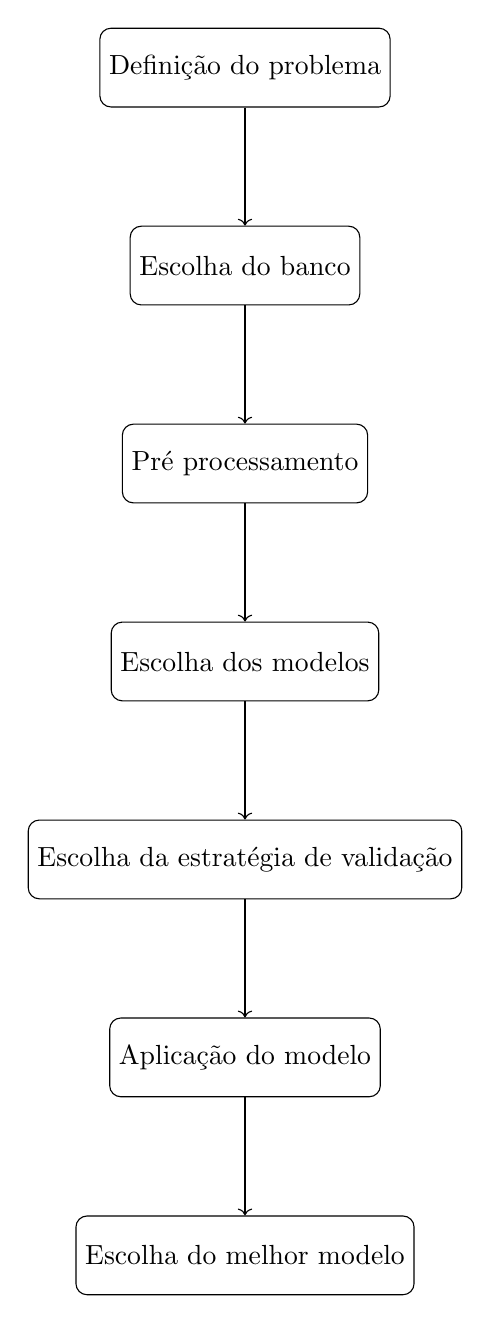
\begin{tikzpicture}[node distance=1.5cm, every node/.style={draw, rounded corners, minimum width=2.8cm, minimum height=1cm, align=center}]

%passos
\node (passo0) {Definição do problema};
\node [below=of passo0] (passo1) {Escolha do banco};
\node [below=of passo1] (passo2) {Pré processamento};
\node [below=of passo2] (passo3) {Escolha dos modelos};
\node [below=of passo3] (passo4) {Escolha da estratégia de validação};
\node [below=of passo4] (passo5) {Aplicação do modelo};
\node [below=of passo5] (passo6) {Escolha do melhor modelo};

%conexões
\draw[->](passo0) -- (passo1);
\draw[->](passo1) -- (passo2);
\draw[->](passo2) -- (passo3);
\draw[->](passo3) -- (passo4);
\draw[->](passo4) -- (passo5);
\draw[->](passo5) -- (passo6);

\end{tikzpicture} % insere o tikzpicture puro
  \label{fig:metodologia}
  \legend{Fonte: Elaborado pelo autor.}
\end{figure}

Cada um desses passos introduz considerações, e as decisões tomadas influenciam nos passos seguintes. Por exemplo, a escolha do banco impacta diretamente em 
quais tipos de pré-processamento necessário, como a limpeza. Contanto, antes mesmo da escolha do banco, é necessário definir qual o problema, visto que 
que as anotações presentes podem limitar o escopo dos problemas resolvidos. 

Nas seções subsequentes, detalha-se as decisões adotadas em cada etapa da metodologia, bem como os critérios considerados para tais escolha.

\section{O banco de dados}
\label{sec:particionamento}

Optou-se pelo \textit{MIT-BIH Arrhythmia Database} \cite{mitbih2005}. Segundo \citeonline{physionet_annotations}, o banco é composto por 58 registros de eletrocardiograma (ECG), cada um com 30 minutos de duração. 
Os 23 primeiros registros, de 100 a 124, foram selecionados aleatoriamente a partir de um conjunto de 4000 gravações de 24 horas realizadas em pacientes ambulatoriais do Beth Israel Deaconess Medical Center. 
Os 25 registros, 200 até 234, restantes foram escolhidos de modo a incluir arritmias raras e com formato complexo, mas clinicamente significativas.
Cada uma das anotações foram feitas com por três cardiologistas independentes. Os sinais foram coletados com duas derivações; uma superior e outra inferior. A superior
é majoritariamente utilizando a derivação MLII (modified limb II) que é feita com o eletrodo no peito. 
Em alguns casos, foi utilizado as derivações V1 (ou mais raramente, V2, V3 e V4); que também são obtidas com os eletrodos no peito.

Neste trabalho, foi utilizado somente a derivação superior, pois permite uma melhor visão do complexo QRS \cite{physionet_annotations}.

Na tabela \ref{tab:mapeamento_classes}, é detalhado o mapeamento entre as classes originais de batimentos para as cinco definidas pela AAMI.

\begin{table}[H]
\centering
\caption{Mapeamento das anotações originais do MIT-BIH para as classes AAMI.}
\label{tab:mapeamento_classes}
\begin{tabular}{ll}
\hline
\textbf{Anotação Original} & \textbf{Classe AAMI} \\
\hline
N, e, j, L, R & N (Normal) \\
A, a, J, S & S (Supraventricular) \\
V, E & V (Ventricular) \\
F, f & F (Fusão) \\
Q, ?, / & Q (Desconhecida) \\
\hline
\end{tabular}
\legend{Fonte: Adaptado de \citeonline{chazal2004}}
\end{table}

O objetivo foi a detecção de batimentos da classe V que compreende: contração prematura ventricular (ou PVC, classe V) e batimento ventricular de escape, classe E, \cite{physionet_annotations}.
Conforme discutido na seção \ref{sub_sec:padroes_arritmias_aami}, apesar de ocorrerem em indivíduos saudáveis, esses tipos arrítmicos possuem relevância clínica pois estão associados a tipos mais graves.

Essas anotações são anotações de batimento, isto é, elas são feitas em cada pico R no ECG. Além delas, existem as anotações de ritmo dentre as quais, podemos destacar: o ritmo normal identificado por (N,
e a taquicardia ventricular; identificado por (VFL. Dentro de um contexto rítmico, podem haver batimentos normais ou arrítmicos.

Por exemplo, na figura \ref{fig:p100_ritmo_normal}, é mostrado o trecho de um ECG. Note a anotação de ritmo, (N, indicando que o mesmo 
é normal. Note, também, que dentro desse contexto rítmico, existem batimentos normais, sinalizados por um ponto em cada pico R, uma arritmia supraventricular,
mais precisamente, o batimento atrial prematuro, classe A.

\begin{figure}[H]
  \centering
  \caption{Trecho ECG com ritmo normal do paciente 100 com arritmia classe A}
  \includegraphics[width=\linewidth]{figuras/ecg_physio_bank/p100_ritmo_normal.png}  % <-- CERTO
  \label{fig:p100_ritmo_normal}
  \legend{Fonte: Adaptado de PhysionNet}
\end{figure}

Na figura \ref{fig:p100_ritmo_normal_arrV} é mostrado um outro trecho do mesmo paciente, o ritmo também é normal

\begin{figure}[H]
  \centering
  \caption{Trecho ECG com ritmo normal do paciente 100 com com arritmia classe V}
  \includegraphics[width=\linewidth]{figuras/ecg_physio_bank/p100_ritmo_normal_classV.png}  % <-- CERTO
  \label{fig:p100_ritmo_normal_arrV}
  \legend{Fonte: Adaptado de PhysionNet}
\end{figure}

Porém, nota-se um PVC, identificado pela anotação V. Na figura \ref{fig:p106_ritmo_normal_arrV}, um trecho do paciente 106 é mostrado.
o ECG é de outro paciente.

\begin{figure}[H]
  \centering
  \caption{Trecho ECG com ritmo normal do paciente 106 com com arritmia classe V}
  \includegraphics[width=\linewidth]{figuras/ecg_physio_bank/p106_ritmo_normal_vt_classV.png}  % <-- CERTO
  \label{fig:p106_ritmo_normal_arrV}
  \legend{Fonte: Adaptado de PhysionNet}
\end{figure}

Aqui temos a ocorrência de uma taquicardia ventricular, identificado por (VT. Nela, ocorrem três PVCs em sequência. 
Note a diferença morfológica entre eles. Após esse evento, o ritmo é normal. Nesse segundo momento, ocorre um outro PVC.

As classes de ritmo não foram utilizadas explicitamente, visto que o objetivo era classificar batimentos. Ou seja, há sequencias 
com ritmo normal ou com taquicardia ventricular, mas o algoritmo não as classifica.

O MIT-BIH é um banco aberto e muito utilizado para a classificação de arritmias, permitindo uma comparação com demais trabalhos.
Além de ser recomendado pela AAMI.

\section{Pré-processamento}
\label{sec:pre_process}

Antes de utilizar o sinal de ECG como entrada dos modelos, foi necessária uma etapa de pré-processamento composta por limpeza de ruídos, 
segmentação e padronização dos batimentos. Essa etapa é importante porque o ECG está sujeito a diversos ruídos que podem prejudicar o 
aprendizado das redes neurais. Como o exame registra a atividade elétrica do coração, correntes elétricas externas ou internas ao organismo 
podem modificar o sinal. Entre os ruídos mais comuns estão o ruído muscular (proveniente da contração de outros músculos), o \textit{baseline wander} 
(variação lenta associada à respiração) e a interferência de 60 Hz da rede elétrica, como discutido na seção \ref{sec:trabalhos_correlatos}.

Apesar disso, alguns trabalhos utilizam o sinal praticamente cru, delegando ao próprio modelo o papel de identificar o que é ou não relevante. 
Essa abordagem simplifica o pré-processamento, mas aumenta a complexidade do problema de aprendizado e pode demandar bases maiores ou arquiteturas 
mais robustas.

Outro desafio importante é a segmentação do ECG em batimentos individuais. Conforme observado nos trabalhos correlatos, existem duas abordagens 
principais: o uso de janelas de tempo fixas ou janelas adaptadas ao tamanho do batimento. Janelas fixas são simples, mas podem cortar partes 
importantes do complexo QRS ou incluir trechos de batimentos vizinhos. Em ambas as estratégias, o pico R é normalmente utilizado como referência. 
Uma vantagem do MIT-BIH é que esses picos já estão anotados; quando não estão, podem ser identificados por algoritmos como o de 
\citeonline{pantompkins1985}.

Neste trabalho, optou-se por trabalhar com o sinal o mais próximo possível do original, preservando suas características fisiológicas e 
facilitando análises posteriores. Por isso, adotou-se a segmentação flexível. Inicialmente, o sinal foi limpo com um filtro passa-alta de 
0,5 Hz (ordem 5), seguido de filtragem da linha de energia a 60 Hz. Em seguida, foi executada a segmentação. Ambas as etapas utilizaram a 
biblioteca NeuroKit2 \cite{Makowski2021neurokit}.

Por fim, foi necessário uniformizar o tamanho dos batimentos antes de alimentá-los nos modelos. A média das amostras por batimento foi de 
aproximadamente 284; portanto, adotou-se uma reamostragem para 288 amostras, correspondendo a 800 ms de duração. Essa etapa foi realizada com a 
função \textit{resample} da biblioteca SciPy \cite{2020SciPy-NMeth}.

Na figura abaixo é ilustrado um batimento segmentado e limpo e o seu trecho correspondente crú.

\begin{figure}[h!]
    \centering
    \caption{Comparação entre o ECG original, segmentado e reamostrado}
    \begin{minipage}{0.5\textwidth}
        \centering
        \includegraphics[width=\linewidth]{figuras/ecg_physio_bank/p101_batimentoSegmentadoVsOrignal.png}
        \subcaption{ECG crú e segmentado}
        \label{fig:image1}
    \end{minipage}%
    \begin{minipage}{0.5\textwidth}
        \centering
        \includegraphics[width=\linewidth]{figuras/ecg_physio_bank/p101_segmentadovsAmostrado.png} 
        \subcaption{ECG segmentado e reamostrado}
        \label{fig:image2}
    \end{minipage}
    \label{fig:twoimages}
    \legend{Fonte: Elaborado pelo autor.}
\end{figure}

\subsection{\textit{Features}}

Após o pré-processamento, é necessário avaliar quais \textit{features} devem ser utilizadas. Em problemas de ECG, essas \textit{features} 
precisam ser relevantes para o domínio clínico. Por outro lado, redes neurais apresentam a vantagem de aprender representações diretamente dos 
dados brutos, o que reduz a necessidade de engenharia manual de atributos. Ainda assim, algumas \textit{features} simples podem complementar o aprendizado, 
fornecendo informação explícita que ajude o modelo a distinguir padrões.

Neste trabalho, optou-se por utilizar apenas o intervalo RR como feature adicional, permitindo que a própria rede aprenda as demais 
características relevantes a partir do sinal segmentado. O intervalo RR é uma informação particularmente útil porque descreve o tempo entre 
batimentos consecutivos. Essa informação ajuda na identificação de arritmias cuja principal manifestação é temporal, como no caso dos batimentos 
ventriculares prematuros (PVCs), em que ocorre um encurtamento característico desse intervalo.

Assim, para um batimento \textit{i}, seu intervalo RR é calculado da seguinte forma.

\begin{equation}
\text{pré RR intervalo} = R_{i-1} - R_{i}
\end{equation}

\begin{equation}
\text{pós RR intervalo} = R_{i} - R_{i+1}
\end{equation}

Note que é necessário saber sobre o próximo batimento, isto é o futuro. Em um contexto de classificação em tempo real, 
por exemplo, isso poderia ser um vazamento, o que não é o caso deste projeto.

\section{Arquiteturas}
\label{sec:modelos}

Após o pré-processamento e a definição das \textit{features}, é necessário escolher as arquiteturas de rede neural que serão avaliadas. 
Como discutido por \citeonline{geron2022hands}, a busca por hiperparâmetros ideais e por configurações de modelo costuma ser um processo 
altamente experimental, podendo incluir técnicas automáticas — como \textit{ grid search} ou \textit{random search} —, mas que, 
no contexto de redes neurais profundas, frequentemente se torna inviável devido ao custo computacional.

Uma alternativa prática consiste em partir de arquiteturas já propostas na literatura e adaptá-las ao problema estudado. 
Seguindo essa estratégia, para o modelo recorrente puro foi adotada como referência a arquitetura apresentada em \citeonline{narotamo2024}. 
No trabalho original, os autores utilizam três camadas de GRUs, cada uma com 256 unidades ocultas, explorando a capacidade das redes recorrentes 
de modelar dependências temporais no sinal.

Neste projeto, a arquitetura base foi mantida, mas além de receber o sinal do eletrocardiograma, o modelo recebeu também os intervalos RR.

A Figura \ref{fig:gru_pura} apresenta um esquema da arquitetura utilizada.

\begin{figure}[H]
  \centering
  \caption{Arquitetura GRU pura.}
  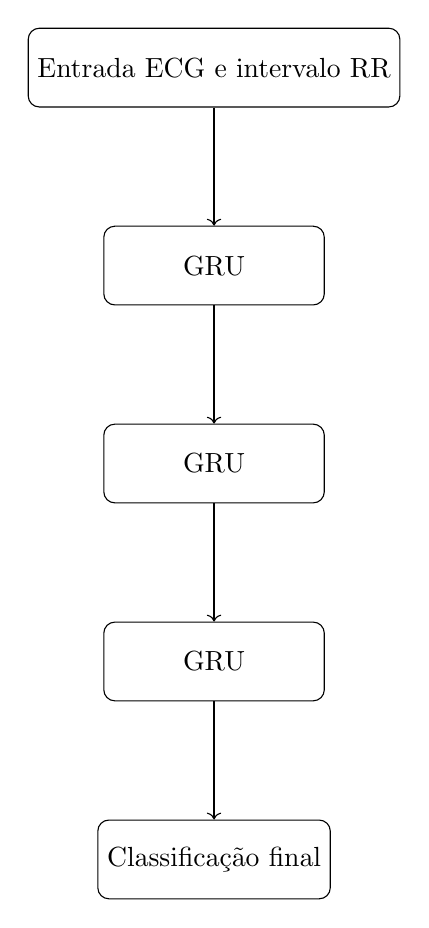
\begin{tikzpicture}[node distance=1.5cm, every node/.style={draw, rounded corners, minimum width=2.8cm, minimum height=1cm, align=center}]

\node (input){Entrada ECG e intervalo RR};
\node [below=of input](gru_1){GRU};
\node [below=of gru_1](gru_2){GRU};
\node [below=of gru_2](gru_3){GRU};
\node [below=of gru_3](saida){Classificação final};

%conexões:

\draw[->](input) -- (gru_1);
\draw[->](gru_1) -- (gru_2);
\draw[->](gru_2) -- (gru_3);
\draw[->](gru_3) -- (saida);
\end{tikzpicture}
 % insere o tikzpicture puro
  \label{fig:gru_pura}
  \legend{Fonte: Elaborado pelo autor.}
\end{figure}

A segunda arquitetura avaliada é um modelo híbrido composto por camadas convolucionais seguidas de uma camada recorrente do tipo GRU. Nessa abordagem, o bloco convolucional é aplicado individualmente a cada batimento da sequência, gerando para cada um deles um mapa de \textit{features} que, em seguida, compõe a nova sequência processada pelo bloco recorrente.

O bloco convolucional é formado por duas camadas de CNN: a primeira com 32 filtros e \textit{kernel} de tamanho sete, e a segunda com 64 filtros e \textit{kernel} de tamanho cinco, ambas utilizando \textit{padding} adequado para preservar o comprimento da entrada. A escolha do tamanho do filtro, ou \textit{kernel}, 
envolve a escolha entre padrões globais, com um \textit{kernel} maior, ou padrões mais locais, com um \textit{kernel} menor. Arquiteturas profundas costumam usar kernels pequenos. Como esta tem apenas duas camadas, foi utilizado um de tamanho sete, e outro de tamanho cinco.

Cada camada convolucional é seguida por \textit{batch normalization} — para estabilizar o treinamento — e por \textit{global max pooling}, que reduz a dimensionalidade do mapa de \textit{features} e contribui para mitigar sobreajuste ao reter apenas as ativações mais relevantes.

A etapa recorrente é composta por uma camada GRU com 256 unidades, responsável por modelar a dependência temporal entre os batimentos por meio das representações produzidas pelo bloco convolucional.

Essa arquitetura representa uma versão simplificada do modelo proposto por \citeonline{narotamo2024}. 

\begin{figure}[H]
  \centering
  \caption{Arquitetura híbrida CNN e GRU.}
  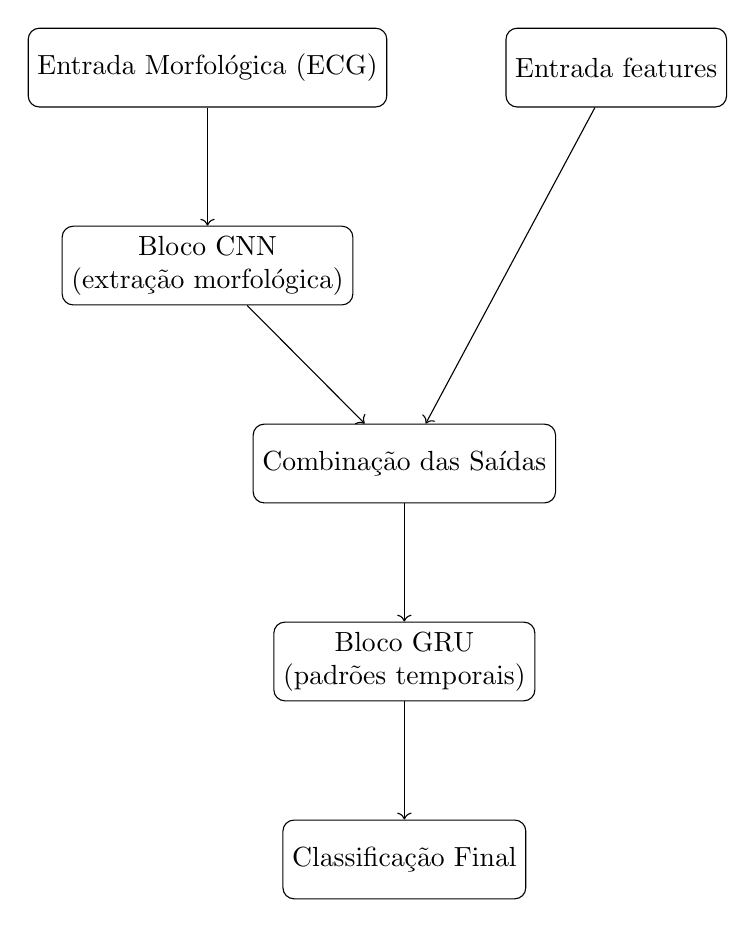
\begin{tikzpicture}[node distance=1.5cm, every node/.style={draw, rounded corners, minimum width=2.8cm, minimum height=1cm, align=center}]

% Entradas
\node (morf) {Entrada Morfológica (ECG)};
\node[right=of morf] (ritmo) {Entrada features};

%blocos de redes neurais:
\node[below=1.5cm of morf] (cnn) {Bloco CNN \\ (extração morfológica)};

% Combinação
\node[below=1.5cm of cnn, xshift=2.5cm] (fusion) {Combinação das Saídas};

% Bloco RNN
\node[below=of fusion] (rnn) {Bloco GRU \\ (padrões temporais)};

%saída
\node[below=of rnn] (saida) {Classificação Final};

%conexões
\draw[->](morf) -- (cnn);
\draw[->](cnn) -- ++ (fusion);
\draw[->](ritmo) -- ++ (fusion);
\draw[->](fusion) -- (rnn);
\draw[->](rnn) -- (saida);

\end{tikzpicture}

 % insere o tikzpicture puro
  \label{fig:cnn_gru}
  \legend{Fonte: Elaborado pelo autor.}
\end{figure}

Enquanto que a rede da figura \ref{fig:gru_pura} recebeu o ECG concatenado com as \textit{features}, a rede híbrida as recebeu separadas, sendo conectadas após o processamento
das CNNs já que o objetivo era que esta extraísse \textit{features} morfológicas.

\subsection{Tamanho da sequência}

Para otimizar o processo de treinamento, foram empregados os mecanismos de \textit{early stopping} e \textit{reduce on plateau}, responsáveis por limitar o número de épocas e ajustar dinamicamente a taxa de aprendizagem, respectivamente. Ambos monitoraram o \textit{f1-score}, de forma que a rede buscasse um equilíbrio entre precisão e \textit{recall}. Assim, mesmo após o treinamento, era possível ajustar manualmente esse compromisso com auxílio da curva PR.

Em ambos os modelos, utilizou-se uma sequência composta por 16 batimentos, sendo a classificação realizada apenas no último elemento da sequência. Dessa forma, o problema caracteriza-se como uma tarefa de sequência para vetor, conforme discutido na Seção~\ref{sec:fundamentos_rnn}.

A escolha do tamanho da sequência foi feita empiricamente. Inicialmente, avaliou-se uma arquitetura simples — uma única camada de LSTM com 100 unidades — utilizando uma validação cruzada one hold out. Embora validações com mais \textit{folds} reduzam o viés na estimativa de generalização, conforme \citeonline{james2023}, o custo computacional cresce proporcionalmente, o que motivou a escolha desse arranjo mais enxuto para experimentação inicial.

Foram testadas sequências de 10, 16 e 20 batimentos. Houve melhora de desempenho ao passar de 10 para 16 batimentos, porém o aumento para 20 resultou em um consumo de memória excessivamente elevado, sem ganho proporcional. Por esse motivo, definiu-se o tamanho final da sequência como 16 batimentos.

As redes foram treinadas por até 50 épocas.

\section{Estratégia de avaliação}

Em seguida, é preciso escolher uma estratégia de avaliação. Conforme apresentado na seção \ref{sec:trabalhos_correlatos},
existem duas estratégias principais: a interpaciente e a intra-paciente. Na primeira, o modelo é exposto a um cenário mais realista,
ele precisa classificar ECG inéditos. O desafio reside justamente na variabilidade dos tipos arrítmicos. Assim, \citeonline{chazal2004}
propôs dois conjuntos de dados para o MIT-BIH; o Ds1 que é formado por: 101, 106, 108, 109, 112, 114, 115, 116, 118, 119, 122, 124, 201, 203, 205, 207, 208, 209, 215, 220, 223 e 230
e o Ds2, formado por: 100, 103, 105, 111, 113, 117, 121, 123, 200, 202, 210, 212, 213, 214, 219, 221, 222, 228, 231, 232, 233 e 234.

Note que o conjunto Ds1 inclui 12 registros que são resultados da seleção aleatória e 10 dos registros com as morfologias complexas. Já no Ds2 possui 
oito dessa primeira seleção e 14 da segunda; sendo mais desafiador e feito para testar a capacidade de generalização do modelo.

Na tabela \ref{tab:particionamento}, é mostrado a distribuição das cinco classes nos dois conjuntos.

\begin{table}[htb]
\centering
\caption{Distribuição das classes nos conjuntos Ds1 e Ds2}
\label{tab:particionamento}
\begin{tabular}{|l|c|c|c|c|c|c|}
\hline
Conjunto & N & SVEB & VEB & F & Q & Total \\ \hline
DS1 & 45 866 & 944 & 3 788 & 415 & 8 & 51 021 \\ \hline
DS2 & 44 259 & 1 837 & 3 221 & 388 & 7 & 49 712 \\ \hline
Total & 90 125 & 2 781 & 7 009 & 803 & 15 & 100 733 \\ \hline
\end{tabular}
\legend{Fonte: o autor.}
\end{table}

Como pode ser observado, as classes são desbalanceadas dentro do mesmo conjunto, porém, balanceada entre eles.

A avaliação foi feita utilizando uma avaliação cruzada no conjunto Ds1 inicialmente com duas partições (dois \textit{folds}) e, posteriormente, com cinco partições (cinco \textit{folds}) nos modelos finais, utilizando o particionados
inter-paciente. Esta estratégia permite avaliar o modelo com ECGs de pacientes para o qual ele não foi treinado; sendo mais próximo de um contexto clínico 
e expõe o modelo a mais variação. Além disso, conforme a AAMI, batimentos com marcapasso foram excluídos por serem não representativos.

Na tabela \ref{tab:folds}, abaixo, é mostrado os pacientes em cada \textit{fold}.

\begin{table}[htbp]
    \centering
    \caption{Distribuição dos IDs dos Pacientes por Fold para Conjuntos de Treinamento e Validação}
    \label{tab:folds}
    \small % Reduz o tamanho da fonte da tabela para melhor encaixe
    \begin{tabular}{|>{\centering\arraybackslash}p{1.5cm}|>{\raggedright\arraybackslash}p{7.5cm}|>{\raggedright\arraybackslash}p{5.5cm}|}
        \toprule
        \textbf{Fold} & \textbf{Conjunto de Treinamento} & \textbf{Conjunto de Validação} \\
        \midrule
        1 & 101, 106, 108, 109, 112, 114, 116, 119, 122, 124, 203, 205, 207, 208, 209, 215, 220, 223 & 115, 118, 201, 230 \\
        \midrule
        2 & 101, 108, 109, 112, 114, 115, 116, 118, 119, 201, 203, 205, 207, 208, 209, 215, 220, 223, 230 & 106, 122, 124 \\
        \midrule
        3 & 101, 106, 108, 109, 112, 114, 115, 116, 118, 122, 124, 201, 207, 208, 215, 220, 223, 230 & 119, 203, 205, 209 \\
        \midrule
        4 & 106, 112, 114, 115, 118, 119, 122, 124, 201, 203, 205, 207, 208, 209, 215, 230 & 101, 108, 109, 116, 220, 223 \\
        \midrule
        5 & 101, 106, 108, 109, 115, 116, 118, 119, 122, 124, 201, 203, 205, 209, 220, 223, 230 & 112, 114, 207, 208, 215 \\
        \bottomrule
    \end{tabular}
    \legend{Fonte: o autor.}
\end{table}

\subsection{Métricas}
\label{sec:metricas}

As métricas utilizadas para avaliar o desempenho dos modelos foram: sensibilidade, precisão, acurácia, \textit{F1-score}, AUC (\textit{Area Under the Curve}) e AP (textit{Average Precision}). Esses 
dois últimos são exibidos juntos ao gráficos \textit{ROC} e \textit{PR}, respectivamente. Além da curva de calibração para avaliar o pior cenário.

A sensibilidade representa a capacidade do modelo em identificar corretamente as classes positivas, isto é, os batimentos arrítmicos. Sua equação é dada por:

\begin{equation}
\text{Sensibilidade} = \frac{TP}{TP + FN}
\end{equation}

em que $TP$ são os verdadeiros positivos e $FN$ os falsos negativos.  

A precisão, por sua vez, indica a proporção de batimentos classificados como arrítmicos que realmente pertencem a essa classe:

\begin{equation}
\text{Precisão} = \frac{TP}{TP + FP}
\end{equation}

onde $FP$ representa os falsos positivos. Precisão e sensibilidade estão relacionadas por um \textit{trade-off}. No contexto médico, prioriza-se elevada sensibilidade, ainda que à custa de menor precisão, uma vez que falsos negativos são mais prejudiciais que falsos positivos.  

O \textit{F1-score} é a média harmônica entre precisão e sensibilidade, buscando um equilíbrio entre ambas:

\begin{equation}
\text{\textit{F1-score}} = \frac{2 \cdot \text{Precisão} \cdot \text{Sensibilidade}}{\text{Precisão} + \text{Sensibilidade}}
\end{equation}

A acurácia corresponde ao acerto global do modelo, considerando tanto as classes positivas quanto as negativas:

\begin{equation}
\text{Acurácia} = \frac{TP + TN}{TP + TN + FP + FN}
\end{equation}

A AUC mede a capacidade do modelo em separar as classes positivas das negativas, variando entre 0 e 1. Valores próximos de 1 indicam separação perfeita, enquanto 0,5 corresponde a um modelo com desempenho equivalente ao acaso,
o \textit{baseline}.

Essa métrica é calculada a partir da área sob a curva ROC. Na Figura~\ref{fig:roc_perfect}, é ilustrado a curva ROC de um classificador perfeito.

\begin{figure}[H]
    \centering
    \caption{Curva ROC de um Classificador Perfeito: Comparação com Modelo Aleatório.}
    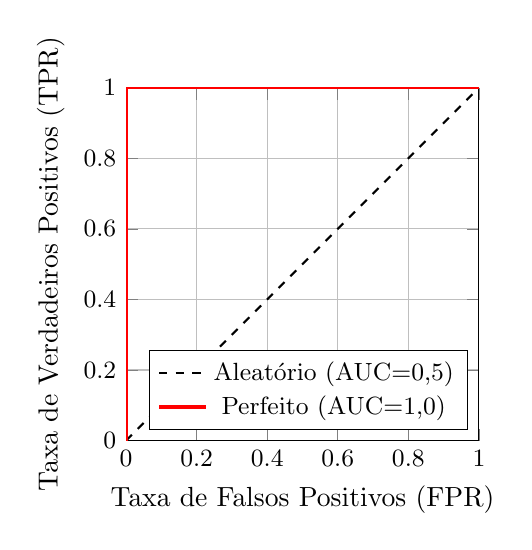
\begin{tikzpicture}
        \begin{axis}[
            width=0.5\textwidth,
            height=0.5\textwidth,
            grid=both,
            xlabel={Taxa de Falsos Positivos (FPR)},
            ylabel={Taxa de Verdadeiros Positivos (TPR)},
            xmin=0, xmax=1,
            ymin=0, ymax=1,
            legend pos=south east,
            legend style={font=\small},
            tick label style={font=\small}
        ]

        % Linha do classificador aleatório
        \addplot[domain=0:1, dashed, thick, color=black] {x};
        \addlegendentry{Aleatório (AUC=0,5)}

        % Curva ROC do Classificador Perfeito
        \addplot[color=red, very thick] coordinates {
            (0,0)  % Inicia
            (0,1)  % Sobe verticalmente até TPR=1, mantendo FPR=0
            (1,1)  % Segue horizontalmente até o fim, mantendo TPR=1
        };
        \addlegendentry{Perfeito (AUC=1,0)}

        \end{axis}
        
    \end{tikzpicture}
    \label{fig:roc_perfect}
    \legend{Fonte: Elaborado pelo autor.}
\end{figure}

A curva vermelha representa um classificador perfeito com TPR, sinônimo de \textit{recall}, sempre igual a um. O raciocínio é que 
para aumentar o \textit{recall}, a quantidade de classes negativas que são classificadas como positivas, calculada por FPR, aumenta. 
Entretanto, para um classificador perfeito, esse \textit{trade-off} não existe.

A linha tracejada representa um classificador aleatório, o \textit{baseline}. Neste caso, por exemplo, para achar 60\% das classes positivas,
cerca de 0,6 de \textit{recall}, o modelo classificaria 60\%  das classes negativas como positivas.

Já a curva PR, Precisão vs \textit{Recall} representa a precisão em função do \textit{recall}. Na figura Figure~\ref{fig:roc_perfect},
é ilustrada a curva PR de um classificador perfeito.

\pgfplotsset{compat=1.18}

\begin{figure}[H]
    \centering
    \caption{Curva Precisão–Recall de um Classificador Perfeito: Comparação com Baseline.}
    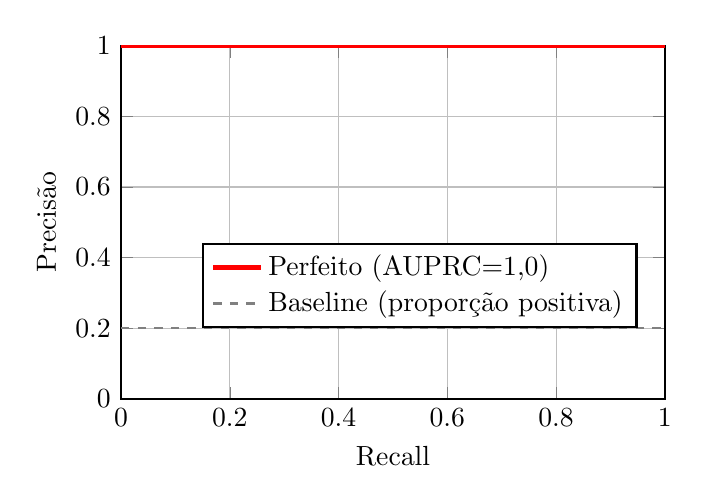
\begin{tikzpicture}
        \begin{axis}[
            width=0.7\textwidth,
            height=0.5\textwidth,
            xlabel={Recall},
            ylabel={Precisão},
            xmin=0, xmax=1,
            ymin=0, ymax=1,
            grid=major,
            legend style={at={(0.95,0.2)},anchor=south east},
            legend cell align={left},
            thick
        ]
        
        % Curva PR do Classificador Perfeito
        \addplot[color=red, ultra thick] coordinates {
            (0.0, 1.0)  % Precisão = 1, Recall = 0
            (1.0, 1.0)  % Precisão = 1, Recall = 1
        };
        \addlegendentry{Perfeito (AUPRC=1,0)}

        % Linha base (baseline) - Mantida como exemplo
        \addplot[dashed, color=gray] coordinates {
            (0,0.2) (1,0.2)
        };
        \addlegendentry{Baseline (proporção positiva)}
        \end{axis}
    \end{tikzpicture}
    
    \label{fig:pr_curve_perfect}
    \legend{Fonte: Elaborado pelo autor.}
\end{figure}

Como há uma relação de \textit{trade-off} entre a precisão e o \textit{recall}, conforme ajusta-se o limiar de decisão para aumentar o \textit{recall},
a precisão tende a cair. Entretanto, assim como ocorre na ROC, esse \textit{trade-off} não existe para um classificador perfeito; ou seja, a precisão é 
sempre 100\% independente do valor do \textit{recall}.

Já a linha tracejada, marca o desempenho de um classificador aleatório; o \textit{baseline}. A linha corresponde a frequência da classe positiva, isto é, 
o classificador aleatório sempre tem uma precisão igual a frequência da classe positiva. AP é o análogo da AUC para esta curva.

Na tabela \ref{tab:matriz_confusao} é ilustrada a matriz de confusão.

\begin{table}[H]
\centering
\caption{Exemplo de matriz de confusão binária}
\label{tab:matriz_confusao}
\begin{tabular}{|c|c|c|}
\hline
\multirow{2}{*}{\textbf{Classe Verdadeira}} & \multicolumn{2}{c|}{\textbf{Classe Predita}} \\ \cline{2-3} 
 & Positiva & Negativa \\ \hline
Positiva & TP & FN \\ \hline
Negativa & FP & TN \\ \hline
\end{tabular}
\legend{Fonte: Elaborado pelo autor.}
\end{table}

Em sentido anti-horário, a partir do canto superior esquerdo temos: 

\begin{enumerate}
\item {TP} \textit{true positive}, quantos casos positivos foram corretamente classificados;
\item {FN} \textit{false negative}, quantos casos positivos foram incorretamente classificados;
\item {FP} \textit{false positive}, quantos casos negativos foram incorretamente classificados;
\item {TN} \textit{true negative}, quantos casos negativos foram incorretamente classificados.
\end{enumerate}

\citeonline{mizilPredictingGoodProbs} apresentam uma definição visual de um modelo perfeitamente calibrado. Em um diagrama de confiabilidade, o modelo é considerado bem calibrado quando, para cada bin de probabilidade, a média das probabilidades previstas corresponde à frequência observada da classe positiva nesse mesmo bin.

Na figura \ref{fig:calibracao_exemplo} é ilustrada um exemplo desse diagrama.

\begin{figure}[ht]
    \centering
    \caption{Diagrama de calibração mostrando curvas de modelos perfeitamente calibrado, superconfiante e subconfiante.}
    \label{fig:calibracao_exemplo}
    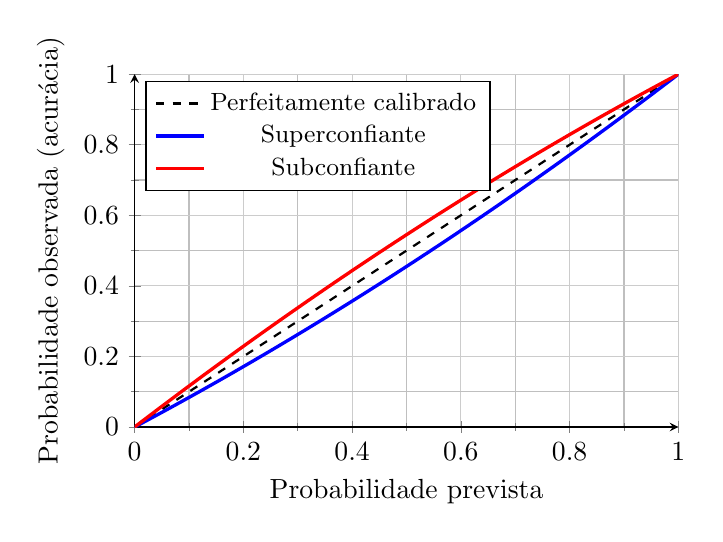
\begin{tikzpicture}
      \begin{axis}[
            width=0.7\textwidth,
            height=0.5\textwidth,
        xmin=0, xmax=1, ymin=0, ymax=1,
        xlabel={Probabilidade prevista},
        ylabel={Probabilidade observada (acurácia)},
        xtick={0,0.2,0.4,0.6,0.8,1},
        ytick={0,0.2,0.4,0.6,0.8,1},
        grid=both,
        major grid style={gray!40},
        minor tick num=1,
        legend style={at={(0.02,0.98)},anchor=north west,font=\small},
        axis lines=left
      ]

      % Linha perfeita (diagonal)
      \addplot [black, thick, dashed, domain=0:1, samples=201] {x};
      % Modelo superconfiante
      \addplot [blue, very thick, domain=0:1, samples=201, smooth] {x - 0.18*x*(1-x)};
      % Modelo subconfiante
      \addplot [red, very thick, domain=0:1, samples=201, smooth] {x + 0.18*x*(1-x)};

      \legend{Perfeitamente calibrado, Superconfiante, Subconfiante}
      \end{axis}
    \end{tikzpicture}
\end{figure}

Um modelo perfeitamente calibrado terá uma curva na diagonal. Logo, caso a probabilidade média prevista seja de 40\%,
então a ocorrência da classe positiva será de 40\%. Um modelo superconfiante terá sua curva abaixo da diagonal, assim, nesse 
mesmo caso, a ocorrência da classe positiva seria abaixo de 40\% e para um modelo subconfiante, a ocorrência da classe positiva 
é maior que a média da probabilidade prevista. 

Os autores explicam que calibração é um aspecto aparte do desempenho, medido pelas demais métricas supracitadas. Muitos contextos,
apenas ter um bom ROC, por exemplo, não é suficiente. Logo, é possível ter um alto desempenho, porém, ter uma calibração ruim.

Essas métricas mostram o desempenho do modelo em perspectivas diferentes, 
precisão, \textit{recall}, \textit{f1 score} e acurácia, mostram o desempenho do modelo para um determinado limiar. Neste trabalho, foi escolhido como 50\%. 
Já as curvas PR e ROC mostram o impacto no desempenho do modelo para diferentes limiares e a matriz de confusão permite visualizar os tipos de erros e acertos
individualmente. A calibração, por outro lado, está relacionada com o quanto as probabilidades previstas refletem a ocorrência real 
dos casos positivos.

\chapter{Resultados e discussões}
\label{ch:resultados}

Nesta seção, serão apresentados os resultados alcançados pelos modelos. Primeiro, a média das métricas com o objetivo de ter uma visão geral do desempenho. 
Em seguida, será feita uma comparação entre as médias na validação com as do treino, para identificar o \textit{overfit}. 
Então, a partir das métricas individuais em cada \textit{fold}, será identificado o pior e o melhor caso de cada modelo utilizando como critério o \textit{f1-score}. 
Apesar do recall ser mais importante, foi adotado o \textit{f1-score} como critério, pois o ajuste no \textit{trade-off} pode ser feito manualmente e a 
critério de um tomador de decisão,
usando a curva ROC ou \textit{precisão-recall}. Em caso de empate será usado o \textit{recall}. 

Para estes casos, será analisada a matriz de confusão, onde poderá ser feito a análise dos tipos de erros e acertos e as curvas de \textit{precisão-recall}, 
para averiguar o impacto da precisão e recall em diferentes \textit{folds} e como os modelos se comparam com o \textit{baseline}.

Então, será eleito o melhor modelo considerando o maior \textit{f1-score} médio. Nesta etapa, é importante analisar também o desvio padrão; é desejável 
que o melhor modelo não tenha apenas um \textit{f1-score} médio alto, mas um desvio padrão baixo, indicando maior estabilidade.

Por fim, será feita a comparação dos modelos com os apresentados na revisão da literatura.

\section{Resultados do modelo GRU}
\label{sec:resultados_gru}

Na Tabela~\ref{tab:resultado_cv_gru_validacao} é mostrado o resultado médio do modelo GRU puro na validação junto com os respectivos desvio padrão.

\begin{table}[H]
\centering
\caption{Média das métricas do GRU para a classificação normal vs. ventricular na validação}
\label{tab:resultado_cv_gru_validacao}
\begin{tabular}{lcc}
\hline
\textbf{Métrica} & \textbf{Média} & \textbf{Desvio Padrão} \\
\hline
Precisão & 0,8515 & 0,1825 \\
\textit{Recall} & 0,8039  & 0,0795 \\
\textit{F1-Score} & 0,8060 & 0,0760 \\
Acurácia & 0,9640 & 0,0278 \\
\hline
\end{tabular}
\legend{Fonte: Elaborado pelo autor.}
\end{table}

Os resultados indicam que o modelo achou aproximadamente 80\% dos casos positivos, com um desvio padrão relativamente baixo, indicando boa estabilidade.
Além disso, a precisão do modelo foi maior que seu \textit{recall}, indicando um perfil mais conservador na classificação. 

A seguir os resultados no treino:

\begin{table}[H]
\centering
\caption{Média das métricas do GRU para a classificação normal vs. ventricular no treino}
\label{tab:resultado_cv_gru_treino}
\begin{tabular}{lcc}
\hline
\textbf{Métrica} & \textbf{Média} & \textbf{Desvio Padrão} \\
\hline
Precisão & 0,9872 & 0,0121 \\
\textit{Recall} & 0,9782 & 0,0150 \\
F1-Score & 0,9827 & 0,0134 \\
Acurácia & 0,9969 & 0,0024 \\
\hline
\end{tabular}
\legend{Fonte: Elaborado pelo autor.}
\end{table}

Comparando os resultados do treino na Tabela~\ref{tab:resultado_cv_gru_cnn_treino} com os resultados da validação na Tabela~\ref{tab:resultado_cv_gru_cnn_validacao},
observa-se um diferença substancial; evidenciando sobreajuste, isto é, o modelo apresentou uma baixa capacidade de generalização para pacientes não vistos.

Esse fenômeno ocorre pois modelos com alta flexibilidade, como redes neurais, conseguem se ajustar intimamente com os dados de treino.
Caso eles não sejam representativos da população, tais modelos podem aprender ruído e particularidades dessa amostra ao invés de padrões generalizáveis.

No contexto do MIT-BIH, o desbalanceamento das classes pode ter causado isso. Como há poucos exemplos da classe positiva, é fácil para o modelo memorizar
padrões morfológicos e rítmicos das arritmias do conjunto de treino, falhando ao encontrar variações dessas instâncias em pacientes diferentes.
Conforme descrito nas seções \ref{sub_sec:padroes_arritmias_aami} e também em \ref{sec:particionamento}, existe uma grande variação 
entre as arritmias, tanto de paciente para paciente quanto intra-paciente.

Outra evidência é a diferença entre a acurácia média do conjunto de treino em relação ao conjunto de validação. Observa-se uma 
diferença significantemente menor. Esta métrica é dominada pela classe negativa, indicando que o modelo conseguiu aprender padrões mais generalizáveis
ao ser exposto a mais exemplos dessa classe. 

Diferente da acurácia, as demais métricas são muito mais sensíveis ao desempenho na classe positiva.

O particionamento usado torna a tarefa de generalização mais desafiadora, pois o modelo é avaliado com ECGs não vistos
durante o treino.

Na Figura~\ref{fig:gru_resultados_por_fold}, está os resultados alcançado pelo modelo em cada \textit{fold} na validação:

\begin{figure}[H]
  \centering
  \caption{Métricas do modelo GRU por \textit{fold}}
   \includegraphics[width=1.0\textwidth]{figuras/modelos_resultados/gru/gru_metricas_por_fold.png} % insere o tikzpicture puro
  \label{fig:gru_resultados_por_fold}
    \legend{Fonte: Elaborado pelo autor.}
\end{figure}

No \textit{fold} três, o modelo obteve sua menor precisão, aproximadamente 0,51 porém obteve um alto \textit{recall}, aproximadamente 0,96.
Essa discrepância sugere que neste \textit{fold}, havia batimentos normais que fugiam do padrão aprendido no treino, fazendo com que o modelo
confundisse eles com batimentos da classe ventricular. Nos demais \textit{folds}, a precisão foi maior que o \textit{recall}, sugerindo a presença 
de arritmias com características mais sutis, que fizeram com que o modelo as confundissem com batimentos normais.

Considerando o \textit{f1-score}, o terceiro \textit{fold} foi eleito o pior. Como o \textit{fold} cinco empatou com o segundo por 
esse mesmo critério, como desempate, aquele com o maior \textit{recall}, o quinto, foi considerado o melhor. 

\subsection{Resultados no pior e melhor caso (Modelo GRU)}

Na Figura~\ref{fig:matriz_confusao_melhor_fold_gru}, está a matriz de confusão do modelo em seu melhor \textit{fold}:

\begin{figure}[H]
  \centering
  \caption{Matriz de confusão do modelo GRU em seu melhor \textit{fold}}
   \includegraphics[width=0.6\textwidth]{figuras/modelos_resultados/gru/matriz_confusao_melhor_fold_gru_alt.png} % insere o tikzpicture puro
  \label{fig:matriz_confusao_melhor_fold_gru}
    \legend{Fonte: Elaborado pelo autor.}
\end{figure}

Na matriz, é possível ver o desbalanceamento das classes. Neste \textit{fold}, o número de sequencias pertencentes a classe
negativa é 9.088, enquanto que 1.384 pertencem a positiva; ou seja, aproximadamente, 13,21\% de todas as sequencias são
da classe positiva. 

A maioria dos erros cometidos são de falsos negativos; o modelo classificou 310 sequencias arrítmicas como normais e 
apenas duas normais como arrítmicas. Algo que já era evidenciado no gráfico \ref{fig:gru_resultados_por_fold}, pois 
sua precisão foi maior que seu \textit{recall}.

%O modelo achou 78\% das arritmias. Porém no pior, como pode ser visto na figura \ref{fig:ap_gru_pior_fold}, o modelo conseguiu achar 96\% das arritmias.
Na Figura~\ref{fig:matriz_confusao_pior_fold_gru}, é dada a matriz de confusão no pior \textit{fold}

\begin{figure}[H]
  \centering
  \caption{Matriz de confusão do modelo GRU em seu pior \textit{fold}}
   \includegraphics[width=0.6\textwidth]{figuras/modelos_resultados/gru/matriz_confusao_pior_fold_gru_alt.png} % insere o tikzpicture puro
  \label{fig:matriz_confusao_pior_fold_gru}
  \legend{Fonte: Elaborado pelo autor.}
\end{figure}

Aqui o desbalanceamento foi mais severo; havia 9.209 classes negativas e 955 classes positivas; 9,39\% aproximadamente. 
Neste \textit{fold}, a situação se inverte: a maioria dos erros foram de falsos positivos, confirmando o que foi visto no 
gráfico \ref{fig:gru_resultados_por_fold}.

%As duas figuras ilustram como o modelo conseguiu aprender melhor a classe negativa do que a classe positiva; evidenciado pelo fato dele confundir
%muito menos negativo com positivo do que o contrário. Um resultado esperado devido a essa ser a classe dominante em todos os \textit{folds}.

\iffalse
A seguir, na figura \ref{fig:roc_cnn_gru_melhor_fold}, a curva ROC no melhor \textit{fold}. Conforme discutido na seção \ref{sec:metricas},
esta curva mostra os diferentes valore do \textit{recall} e do FRP para todos os possíveis limiares de decisão.

\begin{figure}[H]
  \centering
  \caption{Curva \textit{ROC} modelo GRU em seu melhor \textit{fold}}
   \includegraphics[width=0.6\textwidth]{figuras/modelos_resultados/gru/roc_gru_melhor_fold.png} % insere o tikzpicture puro
  \label{fig:roc_melhor_fold_gru}
  \legend{Fonte: Elaborado pelo autor.}
\end{figure}

Considerando que o \textit{baseline}, um classificador aleatório, tem uma \textit{AUC} de 0,5, o melhor foi significantemente melhor.
O gráfico mostra ainda que o modelo consegue ter um \textit{recall} de quase 80\% ao custo de um FPR de 0\%; ou seja, ele não comete 
erros de falso positivo. Para além desse valor, o modelo começaria a cometer tais erros, aumentando o FPR.

\begin{figure}[H]
  \centering
  \caption{Curva \textit{ROC} do modelo GRU em seu pior \textit{fold}}
   \includegraphics[width=0.6\textwidth]{figuras/modelos_resultados/gru/roc_gru_pior_fold.png} % insere o tikzpicture puro
  \label{fig:roc_pior_fold_gru}
  \legend{Fonte: Elaborado pelo autor.}
\end{figure}

No pior fold, \ref{fig:roc_pior_fold_gru}, o modelo ainda conseguiu manter uma performance satisfatória, com um \textit{AUC} de 0,93. 
Neste caso, o modelo tem um \textit{recall} de quase 100\% enquanto mantém um FPR de menos de 20\%. Além desse valor, o \textit{recall}
cresce devagar conforme o erro aumenta, comportamento diferente do observado no pior caso.

Entretanto, devido ao desbalanceamento dos conjuntos, o desempenho pode ser melhor analisado com a curva PR. Conforme a seção \ref{sec:metricas},
esse gráfico mostra os diferentes valores do \textit{recall} e da precisão para todos os possíveis limiares de decisão.
\fi

Na Figura~\ref{fig:ap_cnn_gru_pior_fold} é ilustrada a curva PR do modelo em seu pior \textit{fold}. Conforme a seção~\ref{sec:metricas},
este gráfico mostra os diferentes valores do \textit{recall} e da precisão para todos os possíveis limiares de decisão.

\begin{figure}[H]
  \centering
  \caption{Curva precisão vs \textit{recall} do modelo GRU em seu pior \textit{fold}}
   \includegraphics[width=0.6\textwidth]{figuras/modelos_resultados/gru/ap_gru_pior_fold.png} % insere o tikzpicture puro
  \label{fig:ap_gru_pior_fold}
  \legend{Fonte: Elaborado pelo autor.}
\end{figure}

O \textit{baseline} no pior caso foi de aproximadamente 9,39\%, contrastando com o 49\% alcançado pelo modelo. Entretanto, a precisão foi baixa. Pelo gráfico, é possível ver que, por exemplo, seria 
possível ter um recall de 80\% porém com uma precisão menor que 60\%; ou seja, o modelo encontra 80\% das arritmias, porém, menos de 60\%
de todas as sequências classificadas como arrítmicas realmente são arrítmicas. Neste \textit{fold}, a AUC foi 0,93, maior que o 
\textit{baseline} de 0,5.

Na Figura~\ref{fig:ap_gru_melhor_fold}, ilustra-se a mesma curva porém no melhor \textit{fold}.

\begin{figure}[H]
  \centering
  \caption{Curva precisão vs \textit{recall} do modelo GRU em seu melhor \textit{fold}}
   \includegraphics[width=0.6\textwidth]{figuras/modelos_resultados/gru/ap_gru_melhor_fold.png} % insere o tikzpicture puro
  \label{fig:ap_gru_melhor_fold}
  \legend{Fonte: Elaborado pelo autor.}
\end{figure}

Neste cenário, o modelo alcançou um \textit{AUCPR} de 80\%, enquanto que a proporção de casos positivos foi de 13,21\%.
A precisão do modelo mantém-se alta para \textit{recall} abaixo de 80\%; quase 100\%. Porém, a precisão cai drasticamente, 
menor que 20\%, quando o \textit{recall} ultrapassa essa faixa. 

O AUC do modelo foi de 0,89, maior que o \textit{baseline} de 0,5.

Portanto, apesar do desbalanceamento, o modelo alcançou resultados satisfatórios, considerando o extremo desbalanceamento do conjunto.

\section{Resultados do modelo híbrido GRU e CNN}
\label{sec:resultados_gru_cnn}

O modelo híbrido apresentou resultado superior em relação ao modelo anterior. Na Tabela~\ref{tab:resultado_cv_gru_cnn_validacao}
abaixo, é possível ver que o modelo obteve média maior em todas as métricas. Apesar disso, o modelo obteve um desvio padrão maior 
no \textit{recall} e \textit{F1-score}, mas a diferença foi de apenas 0.0106 e 0.0062, respectivamente.

\begin{table}[H]
\centering
\caption{Média das métricas do modelo híbrido CNN e GRU para a classificação normal vs. ventricular na validação}
\label{tab:resultado_cv_gru_cnn_validacao}
\begin{tabular}{lcc}
\hline
\textbf{Métrica} & \textbf{Média} & \textbf{Desvio Padrão} \\
\hline
Precisão & 0,8800 &  0,1684 \\
\textit{Recall} & 0,8726  & 0,0857 \\
\textit{F1-Score} & 0,8593 & 0,0866 \\
Acurácia & 0,9730 & 0,0258 \\
\hline
\end{tabular}
\legend{Fonte: Elaborado pelo autor.}
\end{table}

Na Tabela~\ref{tab:resultado_cv_gru_cnn_treino}, é possível observar que ainda há \textit{overfit} porém a diferença entre os resultados
do treino e validação do modelo híbrido é menor quando comparado com o modelo GRU puro. Por exemplo, a 
diferença relative entre o \textit{f1-score} de treino e validação para o modelo híbrido foi de aproximadamente 9,56\% 
enquanto que para o modelo recorrente puro, foi de, aproximadamente, 17,98\%.

\begin{table}[H]
\centering
\caption{Média das métricas do modelo híbrido CNN e GRU para a classificação normal vs. ventricular no treino}
\label{tab:resultado_cv_gru_cnn_treino}
\begin{tabular}{lcc}
\hline
\textbf{Métrica} & \textbf{Média} & \textbf{Desvio Padrão} \\
\hline
Precisão & 0,9698 &  0,0180 \\
\textit{Recall} & 0,9313  & 0,0268 \\
\textit{F1-Score} & 0,9502 & 0,0222\\
Acurácia & 0,9915 & 0,0035 \\
\hline
\end{tabular}
\legend{Fonte: Elaborado pelo autor.}
\end{table}

Na Figura~\ref{fig:gru_cnn_resultados_por_fold}, estão os resultados obtidos pelo modelo híbrido em cada \textit{fold}.

\begin{figure}[H]
  \centering
  \caption{Métricas do modelo híbrido CNN e GRU por \textit{fold}}
   \includegraphics[width=1.0\textwidth]{figuras/modelos_resultados/gru_cnn/gru_cnn_metricas_por_fold.png} 
  \label{fig:gru_cnn_resultados_por_fold}
  \legend{Fonte: Elaborado pelo autor.}
\end{figure}

O modelo manteve a tendencia de ter uma precisão acima do \textit{recall} na maioria dos \textit{folds}. É possível observar também que o modelo
obteve um \textit{recall} maior que o modelo GRU puro em todos os \textit{folds} e uma precisão, no geral, maior ou igual. Sendo as exceções,
os \textit{folds} quatro e cinco, porém a diferença foi de, aproximadamente, 0,01 pontos percentuais. 

A seguir, o desempenho do modelo em seu melhor e pior \textit{fold}. Repetindo os critérios descritos na seção \ref{sec:resultados_gru}, o melhor
\textit{fold} foi o segundo e o pior foi o terceiro.

\subsection{Resultados no pior e melhor caso (Modelo Híbrido)}

Na Figura~\ref{fig:matriz_confusao_cnn_gru_melhor_fold}, é ilustrada a matriz de confusão do modelo em seu melhor \textit{fold}.
Neste cenário, o modelo não cometeu nenhum erro de falso negativo, mas 41 de falso positivo. Além de ter acertado 511 arritmias 
e 3.968 batimentos normais.

\begin{figure}[H]
  \centering
  \caption{Matriz de confusão modelo híbrido CNN e GRU em seu melhor \textit{fold}}
   \includegraphics[width=0.6\textwidth]{figuras/modelos_resultados/gru_cnn/matriz_confusao_melhor_fold_gru_cnn_1_alt.png} 
  \label{fig:matriz_confusao_cnn_gru_melhor_fold}
  \legend{Fonte: Elaborado pelo autor.}
\end{figure}

Como pode ser visto no gráfico; o modelo não cometeu nenhum erro de falso positivo e errou 41 arritmias, classificando-as
como batimentos normais. Neste \textit{fold}, a classe positiva compõe, aproximadamente 12,23\% do total. Assim, sendo 
levemente menos balanceado que o melhor \textit{fold} do modelo GRU puro, que tinha 13,21\% de classes positivas, e com um desempenho superior: com um \textit{f1-score}
de 0,97 contra 0,87. 

Já no pior \textit{fold}, Figura~\ref{fig:matriz_confusao_cnn_gru_pior_fold}, a situação se inverte,
a quantidade de erros de falsos negativos, oito, foi menor que as de falsos positivos, 776, refletindo em um
\textit{recall} maior que a precisão; como foi observado no gráfico \ref{fig:gru_cnn_resultados_por_fold}.

\begin{figure}[H]
  \centering
  \caption{Matriz de confusão modelo híbrido CNN e GRU em seu pior \textit{fold}}
   \includegraphics[width=0.6\textwidth]{figuras/modelos_resultados/gru_cnn/matriz_confusao_pior_fold_gru_cnn_3_alt.png} 
  \label{fig:matriz_confusao_cnn_gru_pior_fold}
  \legend{Fonte: Elaborado pelo autor.}
\end{figure}

Na Figura~\ref{fig:ap_cnn_gru_pior_fold} ilustra a curva PR do modelo híbrido em seu pior caso. Comparando com o pior caso 
do modelo GRU, na Figura~\ref{fig:ap_gru_pior_fold}, o modelo híbrido mantém um \textit{recall} maior para os mesmos valores 
de precisão. Em ambos os casos, a precisão quando o \textit{recall} é maior ou igual a um valor próximo a 100\%, porém no modelo puro, isso 
ocorre bem antes. o AP também foi maior; cerca de 0,55 contra 0,49. No piro caso, o AUC do modelo híbrido foi de 0,95, contra 0,93 do 
modelo GRU puro.

\begin{figure}[H]
  \centering
  \caption{Curva precisão vs \textit{recall} do modelo híbrido CNN e GRU em seu melhor \textit{fold}}
   \includegraphics[width=0.6\textwidth]{figuras/modelos_resultados/gru_cnn/ap_gru_cnn_pior_fold_3.png} 
  \label{fig:ap_cnn_gru_pior_fold}
  \legend{Fonte: Elaborado pelo autor.}
\end{figure}

Já a Figura~\ref{fig:ap_cnn_gru_pior_fold} ilustra o melhor caso do modelo híbrido. O AP foi de 0,96 enquanto que o \textit{baseline} seria de aproximadamente
12,23\% e, além disso, o AP foi maior que o obtido pelo GRU puro; que foi de 0,83.

\begin{figure}[H]
  \centering
  \caption{Curva precisão vs \textit{recall} do modelo híbrido CNN e GRU em seu melhor \textit{fold}}
   \includegraphics[width=0.6\textwidth]{figuras/modelos_resultados/gru_cnn/ap_gru_cnn_melhor_fold_1.png} 
  \label{fig:ap_cnn_gru_melhor_fold}
  \legend{Fonte: Elaborado pelo autor.}
\end{figure}

No melhor caso, o modelo mantém uma precisão próxima de 100\% dentro de uma faixa de \textit{recall} que chega próximo aos 85\%. O AUC
foi de 0,96, maior que o \textit{baseline} de 0,5 e do modelo puro, que foi de 0,89

De modo geral, os modelos exibiram um perfil semelhante em seu pior e melhor caso. No pior, a sensibilidade foi maior, resultados
em maiores erros de falso positivo, como resultado, o \textit{recall} foi alto e a precisão foi baixa. No melhor caso, houve um 
equilíbrio maior e, apesar do \textit{recall} mais baixo, a alta precisão aumentou o \textit{f1-score}.

Esse ganho de desempenho sugere que o uso da CNN para extração de \textit{features} morfológicas pode ter sido uma vantagem. A 
camada recorrente do modelo híbrido não precisou aprendê-las do sinal, apenas precisou se concentrar em como elas se encaixam 
no contexto da sequência.

\section{Conclusão dos resultados}

Nesta seção, foi apresentado os resultados obtidos pelos modelos GRU puro e híbrido. Ambos os modelos apresentaram um caso de \textit{overfit},
evidenciado pela grande diferença entre o desempenho no treino com o da validação. A partir das métricas individuais em cada \textit{fold},
foi identificado o pior e melhor caso. Neste primeiro, ambos os modelos tiveram uma precisão bem menor que seu \textit{recall}, invertendo a 
tendência apresentada nos outros \textit{folds}. O que pode ter sido devido a batimentos normais com características destoantes das aprendidas
no treino, fazendo com que os modelos os confundissem com batimentos arrítmicos. 

Em contextos médicos, é preferível um \textit{recall} maior, pois falsos negativos são mais danosos que um falso positivo; isto é, é melhor
dizer que um batimento normal é arrítmico do que o contrário. Entretanto, uma precisão muito baixa pode indicar que o modelo é 
tão bom quanto um modelo aleatório; o que o tornaria inútil. 

Entretanto, os APs dos modelos no pior caso evidenciou que eles superaram esse \textit{baseline}, indicando que foi aprendido padrões que lhes permitem classificar as arritmias, entretanto, esses padrões ainda não são 
perfeitamente generalizáveis.

Conforme apresentado, existe um desbalanceamento entre as classes. Uma forma de contornar esse problema é o uso de "pesos" na função de 
custo para penalizar mais erros na classe minoritária. Seu uso no modelo GRU puro não surtiu o efeito desejado; o \textit{f1-score}
médio, por exemplo, foi de 0,7750 com desvio padrão de 0,1552 contra 0,8060 e desvio padrão de 0,0760; é menor e mais instável.
Uma hipótese está no seu mecanismo de funcionamento. 
Quando se observa as precisão e \textit{recall} do modelo no treino; nota-se um alto desempenho, ou seja, o modelo "prestou" atenção na 
classe minoritária. Assim, uma possível causa é, na verdade, a possível diferença morfológica entre as arritmias de diferentes pacientes.
Neste sentido, o uso de pesos não ajudaria o modelo.

Por fim, na tabela a seguir é resumido os resultados alcançados pelos modelos e os apresentados na seção \ref{sec:trabalhos_correlatos}.
Devido as diferenças metodológicas, a comparação direta entre os resultados não é possível. Além do mais, devido ao sobreajuste 
observado em ambos os modelos, optou-se por não realizar o teste final no Ds2, pois este é um teste único feito quando 
se tem um modelo com um desempenho satisfatório.

\begingroup % Cria um grupo local para as configurações de fonte
\centering
\footnotesize 

% Definição de larguras
% Calculando as larguras para a coluna p{} manual
% Largura restante = \textwidth - (Largura de l) - (Bordas)
% Colunas: l + p1 + p2 + p3 + p4 + p5
% Vamos alocar 10% para o Trabalho, e 18% para o restante (5 * 0.18 = 90%).

% Coluna Trabalho (Ano) - 10% da largura do texto
\setlength{\colwidthA}{0.18\textwidth} 

% As 5 colunas restantes dividem o 90% restante. 
% (0.9 * \textwidth) / 5 = 0.18\textwidth (aproximadamente)
\setlength{\colwidthB}{0.18\textwidth} % Tipo de Modelo
\setlength{\colwidthC}{0.18\textwidth} % Particionamento
\setlength{\colwidthD}{0.18\textwidth} % Features Incluídas
\setlength{\colwidthE}{0.18\textwidth} % Segmentação do Batimento e Limpeza

% Usamos l (para a primeira) e p{largura} com \raggedright para as demais.
\begin{longtable}{|>{\RaggedRight}p{\colwidthA}|>{\RaggedRight}p{\colwidthB}|>{\RaggedRight}p{\colwidthC}|>{\RaggedRight}p{\colwidthD}|>{\RaggedRight}p{\colwidthE}|>{\RaggedRight}p{\colwidthE}|}
% A RaggedRight (do pacote ragged2e, que você tem) é a versão de parágrafo de \raggedright.

% ---------------------------------
% Definição do Cabeçalho da Tabela
% ---------------------------------

\caption{Resumo dos desempenho dos modelos para a classificação de arritmia (ventricular)}
\label{tab:resultados_trabalhos}\\
\hline
\textbf{Trabalho (Ano)} & \textbf{Dataset} & \textbf{Sensibilidade (\%)} & \textbf{Precisão (\%)} \\
\hline
\endhead % Fim do Cabeçalho (Repete em todas as páginas)

% --------

\multicolumn{6}{|r|}{Continua na próxima página...} \\
\hline
\endfoot % Fim do Rodapé (Aparece em todas as páginas, exceto na última)

% ---------------------------------
% Definição do Rodapé da Última Página
% ---------------------------------
\hline
\endlastfoot % Fim da Tabela

% ---------------------------------
% Conteúdo da Tabela
% ---------------------------------

% O \makecell foi removido, exceto nas células onde há uma quebra manual forte
% mas o longtable com p{} já quebra automaticamente.
% Vamos manter o \makecell[l] para a primeira coluna para garantir o alinhamento
% e a quebra manual (se necessário).
\makecell[l]{de Chazal et al. \\ (2004)} & DS2. & 77,7. & 81,9. \\
\hline
\makecell[l] {Mousavi et al. \\(2019)} & DS2. & 98,98. & 97,40.\\
\hline
\makecell[l] {Li et al.\\(2019)} & DS2. & 92,5.& 97,40.\\
\hline
\makecell[l] {Saadatnejad et al.\\(2020)} & Intrapaciente. & 98,22.& 92,97.\\
\hline
\makecell[l] {Kiranyaz et al. \\(2016)} & Intrapaciente. & 95,0.& 89,5.\\
\hline
\makecell[l] {TCC (GRU)} & Cross-validação 5 folds (ds1). & 80,39.& 85,15.\\
\hline
\makecell[l] {TCC (Híbrido)} & Cross-validação 5 folds (ds1). & 87,26.& 88,0.\\
\end{longtable}
\endgroup

\chapter{Análise de erros no pior \textit{fold}}
\label{ch:analise_erros_pior_fold}

Nesta seção, será apresentada uma breve análise de erros do modelo híbrido em seu pior \textit{fold}. 
Conforme os critérios adotados, o eleito foi o terceiro — para ambos os modelos.

Como o recall foi superior à precisão, supoi-se que a causa esteja relacionada à presença de batimentos normais com características morfológicas atípicas, o que pode ter confundido os modelos.
Assim, o objetivo desta seção é verificar como os erros estão distribuídos em relação aos pacientes e quais características
o ECG dos mesmos têm. Por fim, será apresentado também a curva de calibração do modelo, para visualizar a questão da
calibração do mesmo.

Devido ao fato de redes neurais serem modelos caixa-preta, não é possível afirmar quais características contribuíram para 
os erros, logo, a análise serve apenas para construir uma intuição inicial para os resultados achados.

\section{Análise de erros do modelo híbrido CNN com GRU}
\label{sec:analise_erros_cnn_gru}

Na tabela~\ref{tab:erros_acertos_por_paciente}, a seguir, é possível ver que a maioria dos erros foi oriunda de um paciente, o 203.

\begin{table}[H]
\centering
\caption{Total dos erros e acertos por paciente no \textit{fold} de validação}
\label{tab:erros_acertos_por_paciente}
\begin{tabular}{lcc}
\hline
\textbf{Pacientes} & \textbf{Erros} & \textbf{Acertos}\\
\hline
119 & 0 &  1972 \\
203 & 772  & 2186\\
205 & 11 & 2616\\
209 & 1 & 2606\\
\hline
\end{tabular}
\legend{Fonte: Elaborado pelo autor.}
\end{table}

Aproximadamente, 98,46\% de todos os erros foram desse paciente. O modelo errou em torno de 35,31\% de seus batimentos. Conforme visto na 
figura \ref{fig:matriz_confusao_cnn_gru_pior_fold}, a maioria desses erros são de falsos positivos.

Já no paciente 209, o modelo acertou a única classe positiva que existia. O único erro cometido foi um falso positivo. Já no paciente 
205, o modelo acertou 69 das 71 classes positivas e errou 9 classes negativas, das 2.556. Nesses dois pacientes, a classe positiva 
era extremamente rara, mas em números absolutos, a maioria dos erros foram de falsos positivos.

Segundo as anotações do MIT-BIH, disponíveis em \cite{physionet_annotations}, o paciente 203 é considerado como muito difícil. As anotações ainda citam
a presença de mudança de morfologia no complexo QRS e contrações ventriculares prematuras (PVC) de múltiplas formas.

Como o paciente 203 dominou os erros neste \textit{fold} e para o paciente 119, não houve erros, na próxima seção, a análise 
se concentrar neste dois casos. 

Primeiro, será exibida a matriz de confusão do paciente 203 para ilustrar os tipos de erros e acertos, em seguida 
uma comparação entre os trechos de ECG de ambos os pacientes, para comparar a morfologia e possíveis ruídos, e um 
\textit{scatter-plot} dos intervalos RR, para analisar a taxa cardíaca de ambos os pacientes. Neste gráfico, 
o eixo X representa o intervalo RR anterior e o eixo Y, o subsequente. 

Por fim, a curva de 
calibração, para poder ilustrar o cenário de superconfiança em dois casos distintos; um de alto desempenho e outro de 
desempenho menor.

\subsubsection{Comparação morfológica entre o paciente 203 e 119}

Na figura \ref{fig:matriz_confusao_paciente_mais_dificil}, é mostrada a matriz de confusão desse paciente.

\begin{figure}[H]
  \centering
  \caption{Matriz de confusão do paciente 203}
   \includegraphics[width=0.7\textwidth]{figuras/analise_erros/matriz_confusao_paciente_mais_dificil.png} 
  \label{fig:matriz_confusao_paciente_mais_dificil}
  \legend{Fonte: Elaborado pelo autor.}
\end{figure}

O modelo confundiu seis batimentos ventriculares como normais e 766 normais como ventriculares.

Na figura
\ref{fig:erro_acert_neg_class_paciente_mais_dificil}, é ilustrado duas sequencias desse paciente, na primeira
um falso positivo e na segunda um verdadeiro negativo.

\begin{figure}[H]
  \centering
  \caption{ECG normal do paciente 203}
   \includegraphics[width=1.0\textwidth]{figuras/analise_erros/ecg_erro_acerto_neg_paciente_mais_dificil.png} 
  \label{fig:erro_acert_neg_class_paciente_mais_dificil}
  \legend{Fonte: Elaborado pelo autor.}
\end{figure}

É possível observar a forte presença de ruído em ambos os casos. E a presença de batimentos com a morfologia 
bem deformada; após a amostra 2000 no primeiro gráfico e após a amostra 1000 no segundo. 

O modelo tinha 97\% de confiança que o primeiro ECG era da classe positiva. Logo, não é apenas um erro, mas um erro com 
muita confiança; o que já insinua um cenário de superconfiança. No segundo caso, o modelo tinha 12\% de confiança que a 
sequência pertencia a classe positiva, ou seja, 88\% de chance de ser da classe negativa; um acerto com confiança.

Na figura~\ref{fig:acert_neg_class_paciente_mais_facil}, é ilustrada a sequência normal do paciente mais fácil;

\begin{figure}[H]
  \centering
  \caption{ECG normal do paciente 119.}
   \includegraphics[width=0.7\textwidth]{figuras/analise_erros/ecg_sequencia_normal_neg_paciente_mais_facil.png} 
  \label{fig:acert_neg_class_paciente_mais_facil}
  \legend{Fonte: Elaborado pelo autor.}
\end{figure}

É possível notar uma sequencia mais limpa e com o complexo QRS com morfologia usual. Note em torno da amostra
2000 uma contração prematura ventricular.

Na figura \ref{fig:erro_acert_pos_class_paciente_mais_dificil} é ilustrado duas sequências arrítmicas do paciente 203, a primeiro o modelo errou e a segunda ele acertou:

Em ambos os casos, é observável o ruído presenta na figura \ref{fig:erro_acert_neg_class_paciente_mais_dificil}. O 
último batimento da sequência também apresenta uma morfologia diferente da usual.

\begin{figure}[H]
  \centering
  \caption{ECG arrítmico do paciente 203: acerto e erro}
   \includegraphics[width=1.0\textwidth]{figuras/analise_erros/ecg_erro_acerto_pos_paciente_mais_dificil.png} 
  \label{fig:erro_acert_pos_class_paciente_mais_dificil}
  \legend{Fonte: Elaborado pelo autor.}
\end{figure}

O modelo tinha 16\% de confiança que era um caso da classe positiva, logo, 84\% que era da classe negativa; um erro 
confiante. É possível notar uma morfologia relativamente mais limpa e uniforma, principalmente quando comparada às demais sequências 
apresentadas deste paciente, levando o modelo a confundi-la com uma sequência normal.

Já no segundo caso, o modelo tinha 97\% de confiança que era um caso da classe positiva; sendo um 
acerto com confiança. Nota-se a presença de arritmias ventriculares e um sinal com mais ruído; visualmente,
esta sequência é diferente da anterior.

Na figura \ref{fig:acert_posclass_paciente_mais_facil}, é ilustrada uma sequencia arrítmica do paciente 119.
Observe no último batimento, uma arritmia ventricular.

\begin{figure}[H]
  \centering
  \caption{ECG arrítmico do paciente 119.}
   \includegraphics[width=0.7\textwidth]{figuras/analise_erros/ecg_sequencia_normal_pos_paciente_mais_facil.png} 
  \label{fig:acert_posclass_paciente_mais_facil}
  \legend{Fonte: Elaborado pelo autor.}
\end{figure}

\subsubsection{Comparação temporal entre o paciente 203 e 119}

Na figura \ref{fig:poincarefp}, é ilustrado o gráfico de dispersão de um falso positivo do paciente 209.
Note o último batimento da sequência (o 16º), em relação aos demais, ele ocorreu de forma mais prematura uma vez que se encontra na
região inferior esquerda do gráfico, em comparação a outros batimentos — como o quarto, o oitavo e o décimo. Além disso, o intervalo
entre ele e seu sucessor é menor do que o intervalo em relação ao batimento anterior, o que poderia sugerir um padrão compatível com
um batimento ventricular prematuro (PVC). No entanto, essa interpretação dependeria da frequência cardíaca do paciente, e como
discutido na seção \ref{sub_sec:padroes_arritmias_aami}, não existe um padrão universal de ECG normal.

A figura \ref{fig:poincaretp} mostra um caso de verdadeiro positivo do mesmo paciente. O último batimento também ocorre de forma antecipada, porém sua posição mais próxima à linha de identidade indica que o intervalo com o sucessor é aproximadamente igual ao intervalo com o anterior.

\begin{figure}[h!]
    \centering
    \caption{Scatter plot do paciente 203 de um falso positivo e um verdadeiro positivo.}

    \begin{minipage}{0.9\textwidth}
        \centering
        \includegraphics[width=0.7\linewidth]{figuras/analise_erros/poincare_paciente_mais_dificil_fp.png}
        \subcaption{Falso positivo do paciente 203}
        \label{fig:poincarefp}
    \end{minipage}

    %\vspace{0.5cm} % espaço entre as imagens

    \begin{minipage}{0.9\textwidth}
        \centering
        \includegraphics[width=0.7\linewidth]{figuras/analise_erros/poincare_paciente_mais_dificil_tp.png} 
        \subcaption{Verdadeiro positivo do paciente 203}
        \label{fig:poincaretp}
    \end{minipage}

    \legend{Fonte: Elaborado pelo autor.}
    \label{fig:poincare_fp_tp_maisDificil}
\end{figure}


\iffalse
\begin{figure}[H]
  \centering
  \caption{Scatter plot do paciente 203 de um falso positivo.}
   \includegraphics[width=0.70\textwidth]{figuras/analise_erros/poincare_paciente_mais_dificil_fp.png} 
  \label{fig:poicare_fp}
  \legend{Fonte: Elaborado pelo autor.}
\end{figure}

\begin{figure}[H]
  \centering
  \caption{Scatter plot do paciente 203 de um verdadeiro positivo.}
   \includegraphics[width=0.7\textwidth]{figuras/analise_erros/poincare_paciente_mais_dificil_tp.png} 
  \label{fig:poicare_tp}
  \legend{Fonte: Elaborado pelo autor.}
\end{figure}
\fi

Já a figura \ref{fig:poincare_tn_MaisDificil} apresenta um verdadeiro negativo. Embora os pontos estejam igualmente dispersos, o último batimento aparece mais deslocado para o canto inferior direito quando comparado aos dois casos anteriores. Essa diferença pode ter contribuído para que o modelo confundisse o caso negativo anterior como um batimento prematuro, resultando em um falso positivo.

Por fim, a figura \ref{fig:poincare_tn_MaisFacil} mostra uma sequência normal do paciente 119. Diferentemente das anteriores, os batimentos formam agrupamentos mais concentrados, com o último batimento situado próximo ao centro e à linha de identidade.

\iffalse
\begin{figure}[H]
  \centering
  \caption{Scatter plot do paciente 203 de um verdadeiro negativo.}
   \includegraphics[width=0.75\textwidth]{figuras/analise_erros/poincare_paciente_mais_dificil_tn.png} 
  \label{fig:poicare_tn}
  \legend{Fonte: Elaborado pelo autor.}
\end{figure}

\begin{figure}[H]
  \centering
  \caption{Scatter plot do paciente 119 de uma sequência normal.}
   \includegraphics[width=0.7\textwidth]{figuras/analise_erros/poincare_paciente_mais_facil_neg.png} 
  \label{fig:poicare_neg_maisfacil}
  \legend{Fonte: Elaborado pelo autor.}
\end{figure}
\fi

\begin{figure}[h!]
    \centering
    \caption{Scatter plot da sequência normal do paciente 203 e 119}

    \begin{minipage}{0.9\textwidth}
        \centering
        \includegraphics[width=0.7\linewidth]{figuras/analise_erros/poincare_paciente_mais_dificil_tn.png}
        \subcaption{Verdadeiro negativo do paciente 203}
        \label{fig:poincare_tn_MaisDificil}
    \end{minipage}

    %\vspace{0.5cm} % espaço entre as imagens

    \begin{minipage}{0.9\textwidth}
        \centering
        \includegraphics[width=0.7\linewidth]{figuras/analise_erros/poincare_paciente_mais_facil_neg.png} 
        \subcaption{Verdadeiro negativo do paciente 119}
        \label{fig:poincare_tn_MaisFacil}
    \end{minipage}

    \legend{Fonte: Elaborado pelo autor.}
    \label{fig:poincare_normal_maisdificil_maisfacil}
\end{figure}

Para visualizar o quão confiante o modelo foi em seus erros, foi feito a curva de calibração, na figura \ref{fig:curva_calibracao_pior_paciente}, do modelo para o paciente 203 e o paciente 113.

\begin{figure}[H]
  \centering
  \caption{Curva de calibração para o paciente 203 e 119.}
   \includegraphics[width=0.9\textwidth]{figuras/analise_erros/curva_calibracao_pior_paciente_e_melhor_paciente.png} 
  \label{fig:curva_calibracao_pior_paciente}
  \legend{Fonte: Elaborado pelo autor.}
\end{figure}

Em ambos os casos, o modelo foi superconfiante, pois as curvas se mantém a baixo da diagonal principal. Entretanto,
como a curva do paciente 119 se aproxima mais da diagonal, então a para este paciente, a falta de calibração
foi menos severa. Após o \textit{bin} de probabilidade média de 80\%, próximo ao de 100\%, a curva do paciente 119 cruza a diagonal; assim 
o cenário se inverte, o modelo passa a ser pouco confiante.

Para o paciente 203, considerando que em um grupo, o modelo preveja que em média, 90\% deles serão arrítmicos, a realidade é que menos de 60\% deles são. É possível observar,
também, como a superconfiança é mais intensa para \textit{bins} abaixo dos 80\%.

Conforme a discussão da seção \ref{sec:metricas}, a calibração não é diretamente relacionada ao desempenho de um modelo medida pelas métricas usuais.
Isto pode ser observada na curva de calibração do paciente 113 onde o desempenho foi alto, mas a falta de calibração também existe.
Assim, mesmo se o modelo fosse muito sensível e tivesse uma precisão baixa, caso ele fosse bem calibrado, o tomador de decisão poderia 
confiar que as probabilidades previstas seriam mais realista.

\subsubsection{Conclusão da análise de erros}

O objetivo desta seção foi analisar as sequências de batimentos do modelo híbrido em seu pior \textit{fold} para ganhar 
uma intuição adicional às razões da falha do mesmo. Foi identificado que a grande maioria dos erros veio de um único 
paciente, o 203, que as anotações do MIT-BIH o classifica como muito difícil, devido a presença de ruído e arritmias 
atípicas. 

Comparando o paciente 203 com o 119 — paciente para o qual o modelo não cometeu erros — foi identificodo que esse possui 
um sinal mais limpo e sem grandes morfologias atípicas. Além disso, no paciente 203, 
num caso de falso positivo, o intervalo do último batimento da 
em relação ao seu antecessor é mais curto, o que poderia fazer com que o modelo o confundisse com uma arritmia. 

Além disso, a curva de calibração mostrou um cenário de superconfiança para ambos os pacientes, reinforçando a ideia de que 
ela não tem relação direta com o desempenho.

Conforme visto na seção \ref{ch:resultados}, este \textit{fold} também foi o pior caso do modelo GRU e o mesmo ainda se saiu pior que o 
híbrido, com menor \textit{recall} e precisão. O que pode ser outra evidência da vantagem da CNN. Como a CNN atua como extrator de 
\textit{features} da morfologia, ela pode ter mitigado o impacto do ruído e da forma menos usual do ECG deste paciente, resultando 
em um desempenho melhor. Além disso, conforme visto, é possível que os intervalos RR tenha contribuído menos para a separação. Como ambos
os modelos receberam as mesmas \textit{features} RR, então a vantagem da extração feita pela CNN, pode ter ajudado o híbrido a se destacar.



\chapter{Conclusão}

Texto da conclusão.

% Referências (BibTeX)
\bibliographystyle{abntex2-alf}
\bibliography{referencias}

\end{document}
